% Copyright (C) 2024 Songbingzhi628. This work is licensed under Creative Commons Attribution-NonCommercial-ShareAlike 4.0 International License.
% Email: 13012057210@163.com

\ChDecl{Ch4}{4}{}\orMode{\hLk{4O5}{5}\;\;\hLk{4O6}{6}\;\;\hLk{4O7}{7}\;\;\hLk{4O8}{8}\;\;\hLk{4O9}{9}\;\;\hLk{4O10}{10}\;\;\hLk{4O11}{11}\;\;|\;\;\hLk{4O4e2}{4E:\;\;2}\;\;\hLk{4O4e3}{3}\;\;\hLk{4O4e13}{13}}{[1]: (4E 2), 5; [2]: 6, 7, 8, 11; [3]: 9, 10, (4E 13).}

\vspace{3pt}

\BulletPointX\Tips \,\,\,{\tgsl Supp $p\in\PoF{n}$ has at least $n+1$ disti zeros. Then by the ctrapos of [4.12], $\deg p<0\Rightarrow p=0.$}\TextB{}
\Or We show if $p\in\PoFi{}$ has at least $m$ disti zeros, then either $p=0$ or $\deg p\geqslant m.$\TextB{}
If $p=0$ then done. If not, then supp $p$ has exactly $m$ disti zeros $\lambda_1,\dots,\lambda_m.$\TextB{}
Becs $\exists\,!\,\alpha_i\geqslant 1,q\in\PoFi,$ and $q\neq 0,$ suth $p\Par{z}=\Sbra{\Par{z-\lambda_1}{^{\alpha_1}}\cdots\Par{z-\lambda_m}{^{\alpha_m}}}q\Par{z}.$\PfEnd\vspace{2pt}
\BulletPointX\AComm {\tgsl\NOTICE that by [4.17], some term of the poly factoriz might not be in the form $\Par{x-\lambda_k}{^{\alpha_k}}.$}\vspace{-2pt}
\SepLine

\BulletPointX\NoteFor{[4.7]} {\tgsl the uniqnes of coeffs of polys} \hfill[{\tgsc Another proof}]\TextB{\vspace{2pt}}
If a poly had two different sets of coeffs, then
subtracting the two exprs\TextB{}
would give a poly with some nonzero coeffs but infily many zeros. By {\TIPS}.\PfEnd\vspace{-3pt}
\SepLine

\BulletPointX\NoteFor{[4.8]} {\tgsl div algo for polys} \hfill[{\tgsc Another proof}]\TextB{\vspace{-11pt}}
Supp $\deg p\geqslant \deg s$. Then $\FontLarge\BigPar{\FontNorm\underbrace{1, z,\dots, z^{\deg s-1}}_{\text{of\,len}\,\deg s},\overbrace{s,zs,\cdots,z^{\deg p-\deg s}s}^{\text{of\,len}\,\SmallPar{\deg p\,-\,\deg s\,+\,1}}\FontLarge}$ is a bss of $\PoF{\deg p}.$\TextB{\vspace{-7pt}}
Becs $q\in\PoFi,\exists\,!\,a_i,b_j\in\Fbb,$\TextB{}
$q=a_0+a_1 z+\dots+a_{\deg s-1}z^{\deg s-1}+ b_0 s+b_1 zs +\dots+ b_{\deg p-\deg s}z^{\deg p-\deg s}s$\TextB{}
$\Blind{q}=\underbrace{a_0+a_1 z+\dots+a_{\deg s-1}z^{\deg s-1}}_{r}+s\underbrace{\XPar{b_0+b_1 z +\dots+ b_{\deg p-\deg s}z^{\deg p-\deg s}}}_{q}.$ Note that $r,q$ are uniq.\PfEnd[-16pt]
\SepLine

\BulletPointX\NoteFor{[4.11]}\;\;{\tgsl each zero of a poly corres to a deg-one factor;}\hfill[{\tgsc Another proof}]\TextB{\vspace{2pt}}
First supp $p\Par{\lambda}=0.$ Write $p\Par{z}=a_0+a_1 z+\dots+a_m z^m,\exists\,!\,a_0,a_1,\dots,a_m\in\Fbb$ for all $z\in\Fbb.$\vspace{2pt}\TextB{}
Then $p\Par{z}=p\Par{z}-p\Par{\lambda}=a_1\Par{z-\lambda}+\dots+a_m\Par{z^m-\lambda^m}$ for all $z\in\Fbb.$\vspace{2pt}\TextB{}
Hence $\forall k\in\Bra{1,\dots,m},z^k-\lambda^k=\Par{z-\lambda}\Par{ z^{k-1}\lambda^0+ z^{k-2}\lambda^1+\dots+z^{k-\SmallPar{j+1}}\lambda^j+\dots+z\lambda^{k-2}+z^0\lambda^{k-1}}.$\vspace{4pt}\TextB{}
Thus $p\Par{z}=\sum_{j=1}^m a_j \Par{z-\lambda}\sum_{i=1}^k \lambda^{i-1}z^{k-i}=\Par{z-\lambda}\sum_{j=1}^m a_j\sum_{i=1}^k \lambda^{i-1}z^{k-i}=\Par{z-\lambda}q\Par{z}.$\PfEnd
\SepLine

%\BulletPointX\NoteFor{[4.13]}\;\;{\tgsl Every nonconst poly with complex coeffs has a zero in $\Cbb$.} \vspace{2pt}\hfill[{\tgsc Another proof}]\TextB{}
%For any $w\in\Cbb,k\in\Nbp,$ by polar coordinates, $\exists\,r\geqslant 0,\theta\in\Rbb,r\Par{\cos\theta + \i \sin\theta} = w$.\vspace{2pt}\TextB{}
%By De Moivre' theorem, $w^k=\Sbra{r\Par{\cos\theta +\i\sin \theta}}{^k}=r^k\Par{\cos k\theta + \i \sin k\theta}$.\vspace{2pt}\TextB{}
%Hence $\BigPar{r^{1/k}\Par{\cos\frac{\;\theta\;}{k} +\i\sin\frac{\;\theta\;}{k}}}{^k}=w$. Thus every complex number has a {\tgsl $k^{th}$ root}.\vspace{6pt}\TextB{}
%Supp a nonconst $p\in\PoCi$ with highest-order nonzero term $c_m z_m.$\vspace{3pt}\TextB{}
%Then $\aMid{p\Par{z}}\rightarrow\infty$ as $\aMid{z}\rightarrow\infty$ \XPar{ becs $\Frac{\aMid{p\Par{z}}}{\aMid{z_m}}\rightarrow\aMid{c_m}$ as $\aMid{z}\rightarrow\infty$ }.\vspace{3pt}\TextB{}
%\vspace{3pt}Thus the continuous function $z\rightarrow\aMid{p\Par{z}}$ has a global min at some point $\zeta\in\Cbb.$\TextB{}
%\vspace{3pt}To show $p\Par{\zeta} = 0$, asum $p\Par{\zeta}\neq 0$. Define $q\in\PoCi$ by $q\Par{z}=\Frac{p\Par{z+\zeta}}{p\Par{\zeta}}.$\TextB{}
%\vspace{3pt}The function $z\rightarrow\aMid{q\Par{z}}$ has a global min value of $1$ at $z = 0$.\TextB{}
%\vspace{3pt}Write $q\Par{z} = 1 + a_k z^k + \dots + a_m z^m$, where $k\in\Nbp$ is the smallest suth $a_k\neq 0$.\TextB{}
%\vspace{3pt}Let $\beta\in\Cbb$ be suth $\beta^k=-\Frac{1}{a_k}$.\TextB{}
%\vspace{4pt}There is a const $c > 1$ so that if
%$t\in \Par{0, 1}$, then $\aMid{q\Par{t\beta}}\leqslant\aMid{1 + a_k t^k\beta^k}+t^{k+1}c = 1 - t^k \Par{1 - tc}$.\TextB{}
%Now letting $t=1/\Par{2c}$, we get $\aMid{q\Par{t\beta}}<1$. Ctradic. Hence $p\Par{\zeta} = 0$, as desired.\PfEnd
%\SepLine

\ProblemBnoor{\hypertarget{4O4e2}{4E 2}}{
	\TextB{Prove if $w,z\in\Cbb,$ then $\aXMid{\aMid{w}-\aMid{z}}\leqslant\aMid{w-z}.$}
}$\aMid{w-z}{^2}=\Par{w-z}\Par{\overline{w}-\overline{z}}=\aMid{w}{^2}+\aMid{z}{^2}-2Re\Par{w\overline{z}}\geqslant\aMid{w}{^2}+\aMid{z}{^2}-2\aMid{w\overline{z}}=\aXMid{\aMid{w}-\aMid{z}}{^2}.$\vspace{2pt}\parSol{}
\Or $\aMid{w}=\aMid{w-z+z}\leqslant\aMid{w-z}+\aMid{z}\Rightarrow \aMid{w}-\aMid{z}\leqslant\aMid{w-z}.$\parSol{}
\Blind{\Or}$\aMid{z}=\aMid{z-w+w}\leqslant\aMid{z-w}+\aMid{w}\Rightarrow \aMid{z}-\aMid{w}\leqslant\aMid{w-z}.$\PfEnd
\SepLine

\ProblemN{\hypertarget{4O5}{5}}{
	\TextN{Supp $m\in\Nbb,$ and $z_1,\dots,z_{m+1}$ are disti in $\Fbb,$ and $w_1,\dots,w_{m+1}\in\Fbb.$}
	\TextN{Prove $\exists\,!\,p\in\PoF{m},p\Par{z_k}=w_k$ for each $k\in\Bra{1,\dots, m+1}.$}
}\par\quad
Define $T\in\Lm[\BigPar]{\PoF{m},\Fbb^{m+1}}$ by $Tq=\BigPar{q\Par{z_1},\dots,q\Par{z_m},q\Par{z_{m+1}}}.$\vspace{1pt}\par\quad
Becs $Tq=0\Longleftrightarrow q\Par{z_1}=\dots=q\Par{z_m}=q\Par{z_{m+1}}=0\Longleftrightarrow q=0,$ by {\TIPS}. \;Now $T$ iso. Immed.\PfEnd\vspace{4pt}\quad
\Or Let $p_1=1,\;p_k\Par{z}=\prod_{i=1}^{k-1}\Par{z-z_i}=\Par{z-z_1}\cdots\Par{z-z_{k-1}}$ for each $k\in\Bra{2,\dots,m+1}.$\vspace{1pt}\par\quad
By (2.C.10), $B_p=\Par{p_1,\dots,p_{m+1}}$ is a bss of $\PoF{m}.$ Let $B_e=\Par{e_1,\dots,e_{m+1}}$ be the std bss of $\Fbb^{m+1}.$\vspace{2pt}\par\quad
Now $Tp_1=\Par{1,\dots,1},\;Tp_k=\XPar{\prod_{i=1}^{k-1}\Par{z_1-z_i},\dots,\prod_{i=1}^{k-1}\Par{z_j-z_i},\dots,\prod_{i=1}^{k-1}\Par{z_{m+1}-z_i}};$\vspace{3pt}\par\quad
{\normalsize$\begin{pmatrix}
		1 &\hspace{-6pt} 0 &\hspace{-6pt} 0 &\hspace{-6pt} \cdots &\hspace{-6pt} 0\\[-2pt]
		1 &\hspace{-6pt} A_{2,2} &\hspace{-6pt} 0 &\hspace{-6pt} \cdots &\hspace{-6pt} 0\\[-2pt]
		1 &\hspace{-6pt} A_{3,2} &\hspace{-6pt} A_{3,3} &\hspace{-6pt} \cdots &\hspace{-6pt} 0\\[-2pt]
		\vdots &\hspace{-6pt} \vdots &\hspace{-6pt} \vdots &\hspace{-6pt} \ddots &\hspace{-6pt} \vdots\\[-2pt]
		1 &\hspace{-6pt} A_{m+1,2} &\hspace{-6pt} A_{m+1,3} &\hspace{-6pt} \cdots &\hspace{-6pt} A_{m+1,m+1}
	\end{pmatrix}$}${}=\Mt[\BigPar]{T,B_p,B_e}.$ Where $A_{j,k}=\prod_{i=1}^{k-1}\Par{z_j-z_i}\neq 0$ for all $j> k-1\geqslant 1.$\vspace{-74pt}\par\quad
\hfill And $\prod_{i=1}^{k-1}\Par{z_j-z_i}=0 \Longleftrightarrow j\leqslant k-1,$ becs $z_1,\dots,z_{m+1}$ are disti.\Blind{\quad\qquad}\vspace{30pt}\par\quad
\hfill Now the rows $\Mt{T}$ are liney indep. By (4E 3.C.17) \OR (3.F.32).\Blind{\quad}\PfEnd\vspace{3pt}
\SepLine

%\ProblemN[]{\hypertarget{4O4}{4}}{
%	For $m,n\in\Nbp$ with $m\leqslant n,\;\lambda_1,\dots,\lambda_m\in\Fbb,$ let $p\Par{z}=\Par{z-\lambda_1}{^{n-\SmallPar{m-1}}}\Par{z-\lambda_2}\cdots\Par{z-\lambda_m}\Rightarrow\deg p=n.$\TextN{}
%}\SepLine

%\ProblemN{\hypertarget{4O2}{2}}{
%	\TextN{Supp $m\in\Nbp$. Is the set $U=\zeroSubs\cup\Bra{p\in\PoFi:\deg p = m}$ a subsp of $\PoFi$?}
%}$x^m,x^m+x^{m-1}\in U$ \,\,but\,\, $\Deg\Sbra{\Par{x^m+x^{m-1}}-\Par{x^m}}\neq m\Rightarrow \Par{x^m+x^{m-1}}-\Par{x^m}\not\in U.$\PfEnd
%\SepLine
%
%\ProblemN{\hypertarget{4O3}{3}}{
%	\TextN{Supp $m\in\Nbp$. Is the set $U=\zeroSubs\cup\Bra{p\in\PoFi:2\;\mmid\,\deg p}$ a subsp of $\PoFi$?}
%}$x^2,x^2+x\in U$ \,\,but\,\, $\Deg\Sbra{\Par{x^2+x}-\Par{x^2}}$ is odd and hence $\Par{x^2+x}-\Par{x^2}\not\in U.$\PfEnd
%\SepLine

\ProblemN{\hypertarget{4O6}{6}}{
	\TextN{Supp nonzero $p\in\PoF{m}$ has deg $m.$ Prove}
	\TextN{[P] $p$ has $m$ disti zeros $\Longleftrightarrow p$ and its deri $p\apostrophe$ have no common zeros. [Q]}
}(a) Supp $p$ of deg $m$ has $m$ disti zeros. By [4.14], $p\Par{z}=c\Par{z-\lambda_1}\cdots\Par{z-\lambda_m}.$\vspace{1pt}\parSol{\Ha}
If $m=0,$ then $p=c\neq 0\Rightarrow p$ has no zeros, and $p\apostrophe=0,$ done.\parSol{\Ha}
If $m=1,$ then $p\Par{z}=c\Par{z-\lambda_1},$ and $p\apostrophe=c$ has no zeros, done.\vspace{1pt}\parSol{\Ha}
For each $j\in\Bra{1,\dots,m}$, let $q_j\Par{z-\lambda_j}=p\Par{z}\Rightarrow q_j\Par{\lambda_j}\neq 0.$\vspace{1pt}\parSol{\Ha}
Now $p\apostrophe\Par{z}=\Par{z-\lambda_j}q_j\apostrophe\Par{z}+q_j\Par{z}\Rightarrow p\apostrophe\Par{\lambda_j}=q_j\Par{\lambda_j}\neq 0.$\vspace{4pt}\parSol{\Ha}
\Or ${}^{\neg}Q\Rightarrow{}{^\neg}P:$ \;Supp $p\Par{z}=\Par{z-\lambda}q\Par{z},\;p\apostrophe\Par{z}=\Par{z-\lambda}r\Par{z}.$\parSol{\Ha}
Becs $p\apostrophe\Par{z}=\Par{z-\lambda}q\apostrophe\Par{z}+q\Par{z}\Rightarrow p\apostrophe\Par{\lambda}=q\Par{\lambda}=0\Rightarrow q\Par{z}=\Par{z-\lambda}s\Par{z}.$\parSol{\Ha}
Now $p\Par{z}=\Par{z-\lambda}{^2}s\Par{z}.$ Hence $p$ has strictly less than $m$ disti zeros.\vspace{4pt}\parSol{}
(b) ${}^{\neg}P\Rightarrow{}{^\neg}Q:$ \;Becs $0\neq p\in\PoF{m}.$ Supp all disti zeros are $\lambda_1,\dots,\lambda_M,$ with $M<m.$\parSol{\Hb}
By Pigeon Hole Principle, $\Par{z-\lambda_k}{^{2}}q\Par{z}=p\Par{z}$ for some $\lambda_k\Rightarrow p\apostrophe\Par{\lambda_k}=0=p\Par{\lambda_k}.$\PfEnd
\SepLine

\ProblemN{\hypertarget{4O7}{7}}{
	\TextN{Prove every $p\in\PoRi$ of odd deg has a zero.}
}Using the nota and proof of [4.17]. $\deg p=2M+m$ is odd $\Rightarrow m$ is odd. Hence $\lambda_1$ exis.\PfEnd\vspace{3pt}\parSol{}
\Or Supp $p\in\PoRi$ of odd deg $m.$ Let $p\Par{x}=a_0+a_1 x+\dots+a_m x^m.$\parSol{\vspace{3pt}}
Write $p\Par{x}=x^m\envFontSmall\XPar{${\FontLarge$\frac{a_0}{x^m}$}${}+{}${\FontLarge$\frac{a_1}{x^{m-1}}$}${}+\dots+{}${\FontLarge$\frac{a_{m-1}}{x}$}${}+a_m\envFontSmall}\Rightarrow p\Par{x}$ continuous. Let $\delta=\aMid{a_m}{^{-1}}a_m.$\parSol{\vspace{3pt}}
Then $\lim\limits_{x\rightarrow -\infty}p\Par{x}=-\delta\infty\,;\;\;\lim\limits_{x\rightarrow \infty}p\Par{x}=\delta\infty\Rightarrow p$ has at least one real zero.\PfEnd
\SepLine

\ProblemN{\hypertarget{4O8}{8}}{
	\TextN{Supp $p\in\PoRi.$ Define $Tp:\Rbb\rightarrow\Rbb\,$ by $\Par{Tp}\Par{x}={}${\FontNorm$\MathLeftBrace{l}{\Frac{p\Par{x}-p\Par{3}}{x-3}\;$ if $x\neq 3,\\[4pt]p\apostrophe\Par{3}$\hfill if $x=3.}$}\vspace{-10pt}}
	\TextN{Show {\tgnr\large(a)} $Tp\in\PoRi;$ \, {\tgnr\large(b)} $T\in\Lm[\BigPar]{\PoRi}.$\vspace{0pt}}
}\vspace{2pt}\par\quad
(a) For $x\neq 3,T\Par{x^n}={}${\Large$\frac{x^n\,-\,3^n}{x\,-\,3}$}${}=\sum_{i=1}^n 3^{i-1}x^{n-i}.$\vspace{2pt}\par\quad\Ha
For $x=3,T\Par{x^n}=n3^{n-1}=\sum_{i=1}^n 3^{n-1}=\sum_{i=1}^n 3^{i-1}x^{n-i}.$ \,Now each $T\Par{x^n}=\sum_{i=1}^n 3^{i-1}x^{n-i}\in\PoRi{}.$\par\vspace{8pt}\quad
(b) $T\Par{p+\lambda q}\Par{x}={}${\FontSmall$\hMath{l}{\left\{}{\right|}{
		\Frac{\Par{p+\lambda q}\Par{x}-\Par{p+\lambda q}\Par{3}}{x-3},\;$ if $x\neq 3,\\
		\Par{p+\lambda q}\apostrophe\Par{3},$ \hfill if $x=3\Blind{.}
	}$}${}=\Sbra{T\Par{p}+\lambda T\Par{q}}\Par{x}$ for all $x\in\Rbb.$\PfEnd\vspace{16pt}\quad
\Or (a) Becs $\exists\,!\,q\in\PoRi,p\Par{x}-p\Par{3}=\Par{x-3}q\Par{x}.$ For $x\neq 3,\;q\Par{x}={}${\Large\envFontSmall[\footnotesize]\def\SmallPar{\Par}$\frac{p\SmallPar{x}\,-\,p\SmallPar{3}}{x\,-\,3}$}.\par\quad\Ha
\Blind{\Or}$p\apostrophe\Par{x}=\BigPar{p\Par{x}-p\Par{3}}\apostrophe=q\Par{x}+\Par{x-3}q\apostrophe\Par{x}.$ For $x=3,\;p\apostrophe\Par{3}=q\Par{3}.$ Now $Tp=q.$\vspace{4pt}\par\quad
\Blind{\Or}(b) Let $q_k\Par{x}\Par{x-3}=p_k\Par{x}-p_k\Par{3}.$ Now by (a), $Tp_k=q_k.$\par\quad\Hb
\Blind{\Or}Then $\Par{p_1+\lambda p_2}\Par{x}-\Par{p_1+\lambda p_2}\Par{3}=\Par{x-3}\Par{q_1+\lambda q_2}\Par{x}.$ \,By the uniqnes of $q_1+\lambda q_2.$\PfEnd
\SepLine

\ProblemN{\hypertarget{4O11}{11}}{
	\TextNL{Supp $p\in\PoFi$ with $p\neq 0$. Let $U=\Bra{pq:q\in\PoFi}$.\vspace{1pt}}
	\TextNL{{\tgnr\large(a)} Show $\dim\PoFi\XSlash U = \deg p$; \; {\tgnr\large(b)} Find a bss of $\PoFi\XSlash U$.}
}{\tgsl Note that $pq\neq p\circ q,$ see (4E 3.A.10).} \;Let $\deg p=m$ as precond.\par\quad
If $\deg p=0,$ then $U=\PoFi,\PoFi\XSlash U=\Bra{0+U},$ with the uniq bss $\Par{}.$ \;Supp $\deg p\geqslant 1.$\par\vspace{2pt}\quad
(a) Becs $\forall s\in\PoFi,\exists\,!\,r\in\PoF{m-1},q\in\PoFi\Rightarrow\exists\,!\,pq\in U,\;s=\Par{p}q+\Par{r}\Rightarrow\PoFi=U\oplus\PoF{m-1}.$\vspace{0pt}\par\quad\Ha
By \Sbra{3.E {\NOTEFOR} [3.88, 90, 91]} \OR Define $R\Par{s}=r\Rightarrow\null R=U,$ and $R$ surj. Immed.\par\vspace{2pt}\quad
(b) Let $\Par{1,z,\dots,z^{m-1}}$ be a bss of $\PoF{m-1}.$ By (4E 3.E.14) \OR $\tilde{R}{^{-1}}\!:\PoF{m-1}\rightarrow\PoFi{}\XSlash U$, immed.\PfEnd
\SepLine\pagebreak

\ProblemN{\hypertarget{4O9}{9}}{
	\TextN{Supp $p\in\PoCi$. Define $q:\Cbb\rightarrow\Cbb\,$ by $q\Par{z} = p\Par{z}\overline{p\Par{\overline z}}$. Prove $q\in\PoRi$.\vspace{1pt}}
}By [4.5], $\overline z{^n}=\overline{z^n}.$ \;For any $f\Par{z}=a_nz^n+\dots+a_1z+a_0,\;\overline{f\Par{\overline{z}}}=\overline{a_n}z^n+\dots+\overline{a_1}z+\overline{a_0}.$\parSol{}
Becs $q\Par{z}=p\Par{z}\overline{p\Par{\overline z}}=\overline{p\Par{\overline z}}p\Par{z}=\overline{q\Par{\overline z}}.$ \;Each $c_k=\overline{c_k}\Rightarrow c_k\in\Rbb.$\PfEnd\vspace{6pt}\parSol{}
\Or Becs $q\Par{z}=p\Par{z}\overline{p\Par{\overline z}}=\sum_{k=0}^{2n}\XPar{{\sum_{i+j=k}c_i\overline{c_j}}}\,z^k.$ For each $k\in\Bra{0,\dots,2n},$\vspace{0pt}\parSol{}
$\overline{\sum_{i+j=k}c_i\overline{c_j}}=\sum_{i+j=k}\overline{c_i\overline{c_j}}=\sum_{i+j=k}{c_j}\overline{c_i}=\sum_{i+j=k}c_i\overline{c_j}\in\Rbb.$\PfEnd
\SepLine

\ProblemN{\hypertarget{4O10}{10}}{
	\TextNL{Supp disti $x_0,x_1,\dots,x_m\in\Rbb,$ and $p\in\PoC{m}$ suth each $p\Par{x_k}\in\Rbb.$ Prove $p\in\PoRi$.}
}By {\TIPS} and Exe (5), $\exists\,!\,q\in\PoR{m}$ suth $q\Par{x_k}=p\Par{x_k}.$ Hence $p=q.$\PfEnd\vspace{11pt}\quad
\Or Define $q\Par{x}=\sum_{j=0}^m{}${\Large\envFontSmall[\footnotesize]\def\SmallPar{\Par}$\frac{\SmallPar{x\,-\,x_0}\SmallPar{x\,-\,x_1}\,\cdots\,\SmallPar{x\,-\,x_{j-1}}\SmallPar{x\,-\,x_{j+1}}\,\cdots\,\SmallPar{x\,-\,x_m}}{\SmallPar{x_j\,-\,x_0}\SmallPar{x_j\,-\,x_1}\,\cdots\,\SmallPar{x_j\,-\,x_{j-1}}\SmallPar{x_j\,-\,x_{j+1}}\,\cdots\,\SmallPar{x_j\,-\,x_m}}$}${\,}p\Par{x_j}.$\par\vspace{4pt}\quad
又 Each $x_j,\,p\Par{x_j}\in\Rbb\Rightarrow q\in\PoR{m}.$ \;Becs each $q\Par{x_k}=1\cdot p\Par{x_k}\Rightarrow\Par{q-p}\Par{x_k}=0.$\par\quad
$\Par{q-p}$ has $\Par{m+1}$ zeros. By {\TIPS}, $q-p=0\Rightarrow p=q\in\PoRi.$\PfEnd
\SepLine

\ProblemBnoor{\hypertarget{4O4e13}{4E 13}}{
	\TextB{Supp nonconst $p,q\in\PoCi$ have no common zeros. Let $m = \deg p$, $n = \deg q$.\vspace{1pt}}
	\TextB{Define $T:\PoC{n-1}\times\PoC{m-1}\rightarrow\PoC{m+n-1}$ by $T\Par{r, s} = rp + sq.$ Prove $T$ is inje.\vspace{3pt}}
	\ACoro \TextB{$\exists\,!\,r\in\PoC{n-1},s\in\PoC{m-1}$ suth $rp + sq = 1.$}
}Immed, $T$ is liney. \;Supp $T\Par{r,s}=rp+sq=0.$\par\quad
Then $rp=-sq.$ Becs $p,q$ are \uline{coprime} $\Rightarrow p\:\mmid\:s,$ while $\deg s\leqslant m-1\Rightarrow s=0\Rightarrow r=0.$\PfEnd\vspace{6pt}\quad
\Or Let $\lambda_1,\dots,\lambda_M$ and $\mu_1,\dots,\mu_N$ be the disti zeros of $p$ and $q$ respectly. \NOTICE that $M\leqslant m,N\leqslant n.$\vspace{2pt}\par\quad
By the ctrapos of [4.13], $M=0\Longleftrightarrow m=0\Rightarrow s=0\Longleftrightarrow r=0 \Leftarrow n=0\Longleftrightarrow N=0.$\vspace{2pt}\par\quad
Now supp $M,N\geqslant 1.$ We show $s=0.$ \,{\FontSmall Simlr for $r=0.$ \Or $s=0\Rightarrow r=0.$}\vspace{2pt}\par\quad
Write $p\Par{z}=a\Par{z-\lambda_1}{^{\alpha_1}}\cdots\Par{z-\lambda_M}{^{\alpha_M}}.$ \BigPar{ $\exists\,!\,\alpha_j\geqslant 1,a\in\Fbb.$ } Let $\max\!\Bra{\alpha_1,\dots,\alpha_M}=A.$\vspace{2pt}\par\quad
For each $D\in\Bra{0,1,\dots,A-1},$ let $I_{>D}=\Bra{{I_{D,1}},\dots,{I_{D,\,J_D}}}$ be suth each $\alpha\Sbra{I_{D,j}}=\alpha_{I_{D,j}}\geqslant D+1.$\vspace{2pt}\par\quad
Now $\Bra{M}=I_{>A-1}\subseteq \cdots\subseteq I_{>0}=\Bra{1,\dots,M}.$ Becs $rp+sq=0\Rightarrow\Par{rp+sq}{^{\SmallPar{k}}}=0$ for all $k\in\Nbp.$\vspace{2pt}\par\quad
We use induc by $D$ to show $s{^{\SmallPar{D}}}\BigPar{\lambda\Sbra{I_{D,j}}}=0$ for each $D\in\Bra{0,\dots,A-1}.$\vspace{2pt}\par\quad
\NOTICE that $p{^{\SmallPar{D}}}\BigPar{\lambda\Sbra{I_{D,j}}}=0$ for each $D\in\Bra{0,\dots,A-1}$ and each $I_{D,j}\in I_{>D}.$\hfill(L2)\vspace{2pt}\par\quad
(i) $D=0.$ Each $\Par{rp+sq}\BigPar{\lambda\Sbra{I_{0,j}}}=\Par{sq}\BigPar{\lambda\Sbra{I_{0,j}}}=s\BigPar{\lambda\Sbra{I_{0,j}}}=0.$ Where $q\BigPar{\lambda\Sbra{I_{0,j}}}=0.$\vspace{2pt}\par\quad\Hi
$D=1.$ Each $\Par{r\apostrophe p+rp\apostrophe}\BigPar{\lambda\Sbra{I_{1,j}}}+\Par{s\apostrophe q+sq\apostrophe}\BigPar{\lambda\Sbra{I_{1,j}}}=\Par{s\apostrophe q}\BigPar{\lambda\Sbra{I_{1,j}}}=s\apostrophe\BigPar{\lambda\Sbra{I_{1,j}}}=0.$\vspace{1pt}\par\quad\Hi
\Blind{$D=1.$} Where $p\apostrophe\BigPar{\lambda\Sbra{I_{1,j}}}=0,$ and each $I_{1,j}\subseteq I_{0,j}\Rightarrow s\BigPar{\lambda\Sbra{I_{1,j}}}=0.$\vspace{4pt}\par\quad\Endi
(ii) $2\leqslant D\leqslant A-1.$ Asum $\;s{^{\SmallPar{d}}}\BigPar{\lambda\Sbra{I_{d,j}}}=0$ for each $d\in\Bra{0,1,\dots,D-1}$ and each $\lambda\Sbra{I_{d,j}}\in I_{>d}.$\vspace{2pt}\par\quad\Hii
Each $\Sbra{rp+sq}{^{\SmallPar{D}}}\BigPar{\lambda\Sbra{I_{D,j}}}=\Sbra{\mathC_{D}^D r{^{\SmallPar{D}}}p{^{\SmallPar{0}}}+\dots+\mathC_{D}^d r{^{\SmallPar{d}}}p{^{\SmallPar{D-d}}}+\dots+\mathC_{D}^0 r{^{\SmallPar{0}}}p{^{\SmallPar{D}}}}\BigPar{\lambda\Sbra{I_{D,j}}}$\hfill(L1)\vspace{4pt}\par\quad\Hii
\Blind{Each} $\Blind{\Sbra{rp+sq}{^{\SmallPar{D}}}\BigPar{\lambda\Sbra{I_{D,j}}}=}+\Sbra{\mathC_{D}^D s{^{\SmallPar{D}}}q{^{\SmallPar{0}}}+\dots+\mathC_{D}^d s{^{\SmallPar{d}}}q{^{\SmallPar{D-d}}}+\dots+\mathC_{D}^0 s{^{\SmallPar{0}}}q{^{\SmallPar{D}}}}\BigPar{\lambda\Sbra{I_{D,j}}}$\vspace{4pt}\par\quad\Hii
\Blind{Each} $\Blind{\Sbra{rp+sq}{^{\SmallPar{D}}}\BigPar{\lambda\Sbra{I_{D,j}}}}=\Sbra{\mathC_{D}^D s{^{\SmallPar{D}}}q{^{\SmallPar{0}}}}\BigPar{\lambda\Sbra{I_{D,j}}}.$\; Where each $\lambda\Sbra{I_{D,j}}\in I_{>D}\subseteq I_{D-1,\alpha}.$\vspace{4pt}\par\quad\Hii
Hence $s{^{\SmallPar{D}}}\BigPar{\lambda\Sbra{I_{D,j}}}=0.$ The asum holds for all $D\in\Bra{0,\dots,A-1}.$\vspace{6pt}\par\quad
\NOTICE that $\forall k=\Bra{0,\dots,A-2},s{^{\SmallPar{k}}}$ and $s{^{\SmallPar{k+1}}}$ have zeros $\BigBra{{\lambda\Sbra{I_{k+1,1}},\dots,\lambda\Sbra{I_{k+1,\,J_{k+1}}}}}$ in common.\vspace{2pt}\par\quad
Now $\forall D\in\Bra{1,\dots,A-1},s=s{^{\SmallPar{0}}},\dots,s{^{\SmallPar{D}}}$ have zeros $\BigBra{{\lambda\Sbra{I_{D,1}},\dots,\lambda\Sbra{I_{D,\,J_D}}}}$ in common.\vspace{2pt}\par\quad
Thus $s\Par{z}$ is divisible by $\BigPar{z-\lambda\Sbra{I_{D,1}}}{^{\alpha\def\envFont{\scriptsize}\Sbra{I_{D,1}}}}\cdots\BigPar{z-\lambda\Sbra{I_{D,\,J_D}}}{^{\alpha\def\envFont{\scriptsize}\Sbra{I_{D,\,J_D}}}},$ for each $D\in\Bra{0,\dots,A-1}.$\vspace{2pt}\par\quad
Hence $s\Par{z}=\Sbra{\Par{z-\lambda_1}{^{\alpha_1}}\cdots\Par{z-\lambda_M}{^{\alpha_M}}}\,s_0\Par{z},$ while $\deg s<m=\alpha_1+\dots+\alpha_M.$ Now by {\TIPS}.\PfEnd
\SepLine\pagebreak

\ProblemN{L1}{
	\TextB{Prove $\forall p,q\in\PoFi,k\in\Nbp,\Par{pq}{^{\SmallPar{k}}}=\mathC_{k}^k p{^{\SmallPar{k}}}q{^{\SmallPar{0}}}+\dots+\mathC_{k}^j p{^{\SmallPar{j}}}q{^{\SmallPar{k-j}}}+\dots+\mathC_{k}^0 p{^{\SmallPar{0}}}q{^{\SmallPar{k}}}.$\vspace{2pt}}
}We use induc by $k\in\Nbp.$ \;(i) $k=1.$ $\Par{pq}{^{\SmallPar{1}}}=\Par{pq}\apostrophe=C_{1}^1 p{^{\SmallPar{1}}}q{^{\SmallPar{0}}}+C_{1}^0 p{^{\SmallPar{0}}}q{^{\SmallPar{1}}}.$ \;(ii) $k\geqslant 2.$\vspace{2pt}\par\quad
Asum for $\Par{pq}{^{\SmallPar{k-1}}}=\mathC_{k-1}^{k-1} p{^{\SmallPar{k-1}}}q{^{\SmallPar{0}}}+\dots+\mathC_{k-1}^j p{^{\SmallPar{j}}}q{^{\SmallPar{k-1-j}}}+\dots+\mathC_{k-1}^0 p{^{\SmallPar{0}}}q{^{\SmallPar{k-1}}}.$\vspace{4pt}\par\quad
Now $\Par{pq}{^{\SmallPar{k}}}=\BigPar{\Par{pq}{^{\SmallPar{k-1}}}}\apostrophe=\XPar{{\sum_{j=0}^{k-1}\mathC_{k-1}^{j} p{^{\SmallPar{j}}}q{^{\SmallPar{k-j-1}}}}}\apostrophe=\sum_{j=0}^{k-1}\XSbra{\mathC_{k-1}^{j} \XPar{p{^{\SmallPar{j+1}}}q{^{\SmallPar{k-j-1}}}+p{^{\SmallPar{j}}}q{^{\SmallPar{k-j}}}}}.$\vspace{4pt}\par\quad
\Blind{Now} $\Blind{\Par{pq}{^{\SmallPar{k}}}\!}=\XSbra{\mathC_{k-1}^{0}\XPar{ \uwave{p{^{\SmallPar{1}}}q{^{\SmallPar{k-1}}}}+\boxed{p{^{\SmallPar{0}}}q{^{\SmallPar{k}}}}}}+\XSbra{\mathC_{k-1}^1\XPar{p{^{\SmallPar{2}}}q{^{\SmallPar{k-2}}}+\uwave{p{^{\SmallPar{1}}}q{^{\SmallPar{k-1}}}}}}$\vspace{4pt}\par\quad
\Blind{Now} $\Blind{\Par{pq}{^{\SmallPar{k}}}=}+\dots+\XSbra{\mathC_{k-1}^{j-2}\XPar{ \uline{p{^{\SmallPar{j-1}}}q{^{\SmallPar{k-j+1}}}}+p{^{\SmallPar{j-2}}}q{^{\SmallPar{k-j+2}}}}}+\XSbra{\mathC_{k-1}^{j-1}\XPar{ \uuline{p{^{\SmallPar{j}}}q{^{\SmallPar{k-j}}}}+\uline{p{^{\SmallPar{j-1}}}q{^{\SmallPar{k-j+1}}}}}}$\vspace{4pt}\par\quad
\Blind{Now} $\Blind{\Par{pq}{^{\SmallPar{k}}}=}+\XSbra{\mathC_{k-1}^{j}\XPar{ \uwave{p{^{\SmallPar{j+1}}}q{^{\SmallPar{k-j-1}}}}+\uuline{ p{^{\SmallPar{j}}}q{^{\SmallPar{k-j}}}}}}+\XSbra{\mathC_{k-1}^{j+1}\XPar{p{^{\SmallPar{j+2}}}q{^{\SmallPar{k-j-2}}}+\uwave{p{^{\SmallPar{j+1}}}q{^{\SmallPar{k-j-1}}}}}}$\vspace{4pt}\par\quad
\Blind{Now} $\Blind{\Par{pq}{^{\SmallPar{k}}}=}+\dots+\XSbra{\mathC_{k-1}^{k-2}\XPar{ \uline{p{^{\SmallPar{k-1}}}q{^{\SmallPar{1}}}}+p{^{\SmallPar{k-2}}}q{^{\SmallPar{2}}}}}+\XSbra{\mathC_{k-1}^{k-1}\XPar{ \boxed{p{^{\SmallPar{k}}}q{^{\SmallPar{0}}}}+\uline{p{^{\SmallPar{k-1}}}q{^{\SmallPar{1}}}}}}.$\vspace{4pt}\par\quad
Hence $\Par{pq}{^{\SmallPar{k}}}=\mathC_{k}^0{p{^{\SmallPar{0}}}q{^{\SmallPar{k}}}}+\dots+\XSbra{\mathC_{k-1}^{j}+\mathC_{k-1}^{j-1}}\BigPar{p{^{\SmallPar{j}}}q{^{\SmallPar{k-j}}}}+\dots+\mathC_{k}^{k}{p{^{\SmallPar{k}}}q{^{\SmallPar{0}}}}.$\PfEnd
\SepLine

\ProblemN{L2}{
	\TextB{Supp $\alpha\in\Nbp$ suth $p\Par{z}=\Par{z-\lambda}{^\alpha}q\Par{z}.$ Prove ${p{^{\SmallPar{\alpha-1}}}}\Par{\lambda}=0.$}
}$\Sbra{\Par{z-\lambda}{^\alpha}q\Par{z}}{^{\SmallPar{\alpha-1}}}=\sum_{j=1}^{\alpha-1}\mathC_{\alpha-1}^j\Sbra{\Par{z-\lambda}{^\alpha}}{^j}q^{\SmallPar{\alpha-1-j}}.$ Immed.\PfEnd
\SepLine
\ChEnd\pagebreak


\ChDecl{Ch5A}{5.A}{}\orMode{\hLk{5A2}{2}\;\;\hLk{5A3}{3}\;\;\hLk{5A4}{4}\;\;\hLk{5A6}{6}\;\;\hLk{5A7}{7}\;\;\hLk{5A10}{10}\;\;\hLk{5A11}{11}\;\;\hLk{5A12}{12}\;\;\hLk{5A13}{13}\;\;\hLk{5A14}{14}\;\;\hLk{5A15}{15}\;\;\hLk{5A16}{16}\;\;\hLk{5A18}{18}\;\;\hLk{5A19}{19}\;\;\hLk{5A20}{20}\;\;\hLk{5A21}{21}\;\;\hLk{5A23}{23}\;\;\hLk{5A24}{24}\;\;\hLk{5A26}{26}\;\;\hLk{5A27}{27}\;\;\hLk{5A28}{28}$\\[-4pt]$\hLk{5A29}{29}\;\;\hLk{5A32}{32}\;\;\hLk{5A33}{33}\;\;\hLk{5A34}{34}\;\;\hLk{5A35}{35}\;\;\hLk{5A36}{36}\;\;|\;\;\hLk{5A2e20}{2E:\;20}\;\;|\;\;\hLk{5A4e8}{4E:\;\;8}\;\;\hLk{5A4e11}{11}\;\;\hLk{5A4e15}{15}\;\;\hLk{5A4e16}{16}\;\;\hLk{5A4e17}{17}\;\;\hLk{5A4e36}{36}\;\;\hLk{5A4e37}{37}\;\;\hLk{5A4e39}{39}}[-40pt]{[1]: 2, 3, 6; [2]: 7, 10, 18, 19, 20, 11, 12; [3]: 13, (4E 11), (4E 8), 14, 15, (4E 15), 21;$\\$[4]: (4E 17), 16, 23, (2E 20), (4E 37), 26, 29; [5]: 32, (4E 36), 35, 36, 24; [6]: (4E 16), 27, 28; [7]: (4E 39).}

\vspace{6pt}

\BulletPointX\NoteForSmall{[5.6]}\;\;If $V$ is infinide. Then (a) $\Longleftrightarrow$ (b) $\Rightarrow$ (d), while (b) $\notRightarrow$(c), and (b) $\notRightarrow$(d).\par
\BulletPointX\AComm $\lambda$ not an eigval of $T\Longleftrightarrow{T-\lambda I}$ inje $\Longleftrightarrow$ inv, if finide.
\SepLine

\BulletPointX\Tips \,\,\,Supp $T_1,\dots,T_m\in\Lm{V}.$\TextB{\vspace{-2pt}}
(a) If $T_1,\dots,T_m$ all inje. Then $\Par{T_1\circ\cdots\circ T_m}$ inje. \;Convly true if finide, by (3.D.9).\TextB{}
(b) The ctrapos of (a): If $\Par{T_1\circ\cdots\circ T_m}$ not inje. Then $\exists$ some $T_k$ not inje.\TextB{}
(c) \Sbra[3pt]{{\tgsl Req Infinide}} \;$T_k$ not inje $\notRightarrow\Par{T_1\circ\cdots\circ T_m}$ not inje, unless $k=1$.\TextB{}
\Hc\AExa Forwd and backwd shift optors on $\Fbb^\infty.$
\SepLine

\ProblemB{
	\TextB{Supp $V$ is finide, $T\in\Lm{V},$ and $U$ is invarsp of $\,V$ under $T.$}
	\TextB{Prove or give a countexa\hspace{1pt}$:$ there exis invarsp of dimension $\dim V-dim U.$}
}\parSol{}
\SepLine

\ProblemB[]{
	\TextB{Supp $T\in\Lm{V}$ and $U$ is invarsp of $V$ under $T.$}
	\TextB{Supp $\lambda_1,\dots,\lambda_m$ are the disti eigvals of $T$ corres eigvecs $v_1,\dots,v_m.$}
}
\ProblemB{
	\TipsN{1}\,\,\TextB{Prove $v_1+\dots+v_m\in U\Longleftrightarrow$ each $v_k\in U.$\vspace{-2pt}}
}Supp each $v_k\in U.$ Then becs $U$ is a subsp, $v_1+\dots+v_m\in U.$\parSol{}
Convly, consider the stmt $P\Par{k}:$ if $v_1+\dots+v_k\in U,$ then each $v_j\in U.$\parSol{}
(i) For $k=1,$ $v_1\in U,\;P\Par{1}$ holds.\parSol{\Endi}
(ii) For $2\leqslant k\leqslant m.$ Asum $P\Par{k-1}$ holds. Supp $v=v_1+\dots+v_k\in U.$\parSol{\Hii}
Then $Tv=\lambda_1v_1+\dots+\lambda_k v_k\in U\Longrightarrow Tv-\lambda_k v=\Par{\lambda_1-\lambda_k}v_1+\dots+\Par{\lambda_{k-1}-\lambda_k}v_{k-1}\in U.$\parSol{\Hii}
For each $j\in\Bra{1,\dots,k-1},\lambda_j-\lambda_{k}\neq 0\Rightarrow\Par{\lambda_j-\lambda_k}v_j=v_j'$ is an eigvec of $T$ corres $\lambda_j.$\parSol{\Hii}
By asum, each $v_j'\in U.$ Thus $v_1,\dots,v_{k-1}\in U.$ So that $v_k=v-v_1-\dots-v_{k-1}\in U.$\PfEnd
\SepLine[0pt][\Blind{\BulletPointX} ]

\ProblemB{
	\TipsN{2}\,\,\TextB{Supp $\dim V=m\Rightarrow B_V=\Par{v_1,\dots,v_m}.$ Let each $E_k=\Span{v_k}.$}
	\IndentTipsN{2}\TextB{Prove $U=\BigPar[0pt]{U\cap E_1}\oplus\cdots\oplus\BigPar[0pt]{U\cap E_m}.$\vspace{-1pt}}
}Becs $V=E_1\oplus\cdots\oplus E_m\Rightarrow\forall v\in U,\exists\,!\,c_j\in E_j,v=c_1v_1+\dots+c_mv_m.$\parSol{}
For each $j,$ $c_j\neq 0\Rightarrow c_jv_j$ eigvec corres $\lambda_j.$ Othws $c_jv_j=0\in U.$\parSol{}
By \TIPSN{1}, each $c_jv_j\in U.$ Thus $v\in\Par{U\cap E_1}\oplus\dots\oplus\Par{U\cap E_m}=U.$\PfEnd\vspace{2pt}
\ACoro Becs each $\dim E_j=1\Rightarrow\Par{U\cap E_j}=E_j$ or $\zeroSubs.$ Let $E_{k_1},\dots,E_{k_M}$ be all suth each $E_{k_j}=U\cap E_{k_j}.$\par
\BulletPointX\TipsN{3}\,\,\,{\tgsl Supp $U$ is a nonzero invarsp of $V$ under $T.$ Let $\dim V=m.$ Then $U=\Span{v_{k_1},\dots,v_{k_M}}.$}
\SepLine

\ProblemN{2, 3}{
	\TextB{Supp $S,T\in\Lm{V}$ suth $ST=TS.$ Prove $\null T,\range T$ invard $S.$}
}(a) $Tv=0\Rightarrow TSv=STv=0.$ \;\; (b) $Tu=v\Rightarrow Sv=STu=TSu\in\range T.$\PfEnd
\ACoro For any $\lambda,\mu\in\Fbb,\Null\Par{T-\lambda I},\Range\Par{T-\lambda I}$ is invard $\Par{S-\mu I}.$\vspace{-2pt}
\SepLine

\ProblemN{\hypertarget{5A6}{6}}{
	\TextN{Supp $U$ is invarsp of nonzero $V$ under any $T\in\Lm{V}.$ Show $U=V$ or $\zeroSubs$.}
}We show the ctrapos: {\tgsl Supp $U\neq\zeroSubs$ and $U\neq V.$ Prove $\exists\,T\in\Lm{V},\,U$ is not invard $T$.}\parSol{}
Let $W\oplus U=V.$ Define $T\in\Lm{V}$ by $T\Par{u+w}=w.$\PfEnd
\SepLine
\pagebreak

\BulletPointX\Tips \,\,\,{Supp $T\in\Lm{\Rbb^2}$ is the countclockwise rotation by the angle $\theta\in\Rbb.$}\par\quad
{Define $\mathcal{C}\in\Lm{\Rbb^2,\Cbb}$ by $\mathcal{C}\Par{a,b}=a+\i b=r\Par{\cos\alpha+\i\sin\alpha}\Rightarrow a=r\cos\alpha,b=r\sin\alpha,$ where $r=a^2+b^2.$}\par\quad
{Then $\Par{\cos\theta+\i\sin\theta}\Par{a+\i b}=r\BigPar{\cos\!\Par{\alpha+\theta}+\i\sin\!\Par{\alpha+\theta}}=\mathcal{C}^{-1}T\Par{a,b}.$}\par\quad
{Hence $T\Par{a,b}=\BigPar{a\cos\theta-b\sin\theta,a\sin\theta+b\cos\theta}.$ Now $\Mt{T}=\;${\normalsize$\begin{pmatrix}
			\cos\theta & -\sin\theta\\
			\sin\theta & \Blind{-}\cos\theta
		\end{pmatrix}$}.}\vspace{6pt}\par\quad
\Example \,\,\,\OR\ProblemN[]{\hypertarget{5A7}{7}}{ Supp $T\in\Lm{\Rbb^2}$ is defined by $T\Par{x, y} = \Par{-3y, x}.$ Find all eigvals of $T$.\TextN{\vspace{4pt}}}\quad
\NOTICE that $\Mt{T}=\;${\normalsize$\begin{pmatrix}
		\cos90^\circ & -3\sin90^\circ\\
		\sin90^\circ & \Blind{-}\cos90^\circ
	\end{pmatrix}$}. By [5.8](a), we conclude that $T$ has no eigvals.\vspace{4pt}\par\quad
\Or Supp $\lambda$ is eigval with eigvec $\Par{x,y}.$ Then $\Par{\lambda x,\lambda y}=\Par{-3y,x}\Rightarrow-3y=\lambda^2 y\Rightarrow \lambda^2=-3.$\par\quad
\Blind{\Or}\Sbra{ Ignoring the possibility of $y=0,$ becs $x=0\Longleftrightarrow y=0.$ }\PfEnd
\SepLine

%\ProblemN{\hypertarget{5A8}{8}}{
%	\TextN{Define $T\in\Lm{\Fbb^2}$ by $T\Par{w, z} = \Par{z, w}$. Find all eigvals and eigvecs.}
%}Supp $\lambda$ is an eigval with an eigvec $\Par{w,z}.$ Then $z=\lambda w$ \,{\small and}\, $ w=\lambda z.$\parSol{}
%Thus $z=\lambda^2 z\Rightarrow \lambda^2=1,$ ignoring the possibility of $z=0$ \Par{ $z=0\Longleftrightarrow w=0$ }.\parSol{}
%Hence $\lambda_1=-1$ and $\lambda_2=1$ are all the eigvals of $T.$ And $T\Par{z,z}=\Par{z,z},T\Par{z,-z}=\Par{-z,z}.$\parSol{}
%又 $\dim\Fbb^2=2.$ Thus the set of all eigvecs is $\Bra{\Par{z,z},\Par{z,-z}:z\neq 0}.$\PfEnd
%\SepLine
%
%\ProblemN{\hypertarget{5A9}{9}}{
%	\TextN{Define $T\in\Lm{\Fbb^3}$ by $T\Par{z_1,z_2,z_3}=\Par{2z_2, 0,5z_3}$. Find all eigvals and eigvecs.}
%}Supp $\lambda$ is an eigval with an eigvec $\Par{z_1,z_2,z_3}.$\parSol{}
%Then $\Par{2z_2, 0,5z_3}=\lambda\Par{z_1,z_2,z_3}.$ We discuss in two cases:\parSol{}
%For $\lambda=0,$\, $z_2=z_3=0$ and $z_1$ can be arb \Par{ $z_1\neq 0$ }.\parSol{}
%For $\lambda\neq 0,$\, $z_2=0=z_1,$ and $z_3$ can be arb \Par{ $z_3\neq 0$ }, then $\lambda=5$.\parSol{}
%The set of all eigvecs is $\Bra{\Par{0,0,w},\Par{w,0,0}:w\neq 0}.$\PfEnd
%\SepLine

\ProblemN{\hypertarget{5A10}{10}}{
	\TextNL{Define $T\in\Lm{\Fbb^n}$ by $T\Par{x_1,x_2,x_3,\dots,x_n}=\BigPar{x_1,2 x_2,3 x_3,\dots,n x_n}.$}
	(a) \TextNL{Find all eigvals and eigvecs;\;\; {\tgnr\large(b)} Find all invarsps of $V$ under $T.$}
}Let $\Par{e_1,\dots,e_n}$ be the std bss of $\Fbb^n.$\parSol{}
(a) The eigvals are $\Bra{1,\dots,n}$ of len $\dim\Fbb^n.$ Let each $E_k=\Span{e_k}.$\parSol{\Ha}
The set of all eigvecs is $\Par{E_1\cup\cdots\cup E_n}\nonzero[\Big].$\parSol{}
(b) Let each $V_{\!k}=\Span{e_k}\Rightarrow V_{\!k}$ invard $T.$ Then every sum of $V_{\!1},\dots,V_{\!n}$ is invard $T.$\PfEnd
\SepLine

\ProblemN{\hypertarget{5A18}{18}}{
	\TextNL{Define $T\in\Lm{\Fbb^\infty}$ by $T\Par{z_1,z_2,\cdots}=\BigPar{0, z_1,z_2,\cdots}.$ Show $T$ has no eigvals.}
}Supp $z_k\neq 0$ and $T\Par{z_1,z_2,\dots}=\Par{\lambda z_1,\lambda z_2,\dots}=\Par{0,z_1,z_2,\dots}.$ Thus $\lambda z_1=0,\,\lambda z_k=z_{k-1}.$\parSol{}
($-$) $\lambda=0\Rightarrow\lambda z_2=z_1=0=\dots=z_k\Rightarrow\Par{z_1,z_2,\dots}=0.$ Not an eigval.\parSol{}
($=$) $\lambda\neq 0\Rightarrow\lambda z_1=0\Rightarrow z_1=\dots=z_k=0.$ Not an eigval.\PfEnd
\SepLine

\ProblemN{\hypertarget{5A19}{19}}{
	\TextNL{Supp $n\in\Nbp$. Define $T\in\Lm{\Fbb^n}$ by $T\Par{x_1,\dots,x_n}=\BigPar{x_1+\dots+x_n,\dots,x_1+\dots+x_n}.$}
	\TextNL{\FontNorm In other words, the ent of $\Mt{T}$ wrto the std bss are all \,$1$'s.\; \FontLarge Find all eigvals and eigvecs of $T.$\vspace{-2pt}}
}Supp $x_k\neq 0$ and $T\Par{x_1,\dots,x_n}=\Par{\lambda x_1,\dots,\lambda x_n}=\BigPar{x_1+\dots+x_n,\dots,x_1+\dots+x_n}.$\parSol{}
Then (I) $\lambda=0\Rightarrow x_1+\dots+x_n=0;$ \;(II) $\lambda\neq 0\Rightarrow x_1=\dots=x_n\Rightarrow\lambda x_k=n x_k.$
\SepLine

\ProblemN{\hypertarget{5A20}{20}}{
	\TextNL{Define $S\in\Lm{\Fbb^\infty}$ by $S\Par{z_1,z_2,z_3,\cdots} = \Par{z_2,z_3,\cdots}.$}
	\TextNL{Show every elem of $\Fbb$ is an eigval of $S$, and find all eigvecs of $S$.\vspace{-2pt}}
}Supp $z_k\neq 0$ and $S\Par{z_1,z_2,\dots}=\Par{\lambda z_1,\lambda z_2,\dots}=\Par{z_2,z_3,\dots}.$ Then each $\lambda z_k=z_{k+1}.$\parSol{}
(I) $\lambda=0\Rightarrow$ each$z_k=\dots=z_2=\lambda z_1=0.$ Let $z_1\neq0\Rightarrow E\Par{0,S}=\Span{e_1}.$\parSol{}
(II) $\lambda\neq 0\Rightarrow\lambda^k z_1=\lambda^{k-1} z_2=\dots=\lambda z_k=z_{k+1},$ let $z_1\neq 0\Rightarrow E\Par{\lambda,S}=\Span[\Sbra]{\Par{1,\lambda^1,\cdots,\lambda^k,\cdots}}.$\PfEnd
\SepLine

\ProblemN{\hypertarget{5A11}{11}}{
	\TextNL{Define $T:\PoRi\rightarrow\PoRi$ by $Tp = p\apostrophe$. Find all eigvals and eigvecs.}
}For $0\neq p\in\PoRi,\deg p\apostrophe<\deg p.$ And $\deg 0=-\infty.$ Supp $p\apostrophe=\lambda p.$\parSol{}
Asum $\lambda\neq 0.$ Then $\deg\lambda p=\deg p\apostrophe<\deg\lambda p,$ ctradic. Thus $\lambda=0.$\parSol{}
Therefore $\deg\lambda p=-\infty=\deg p\apostrophe\Rightarrow p\in\PoR{0}.$\PfEnd
\SepLine

\ProblemN{\hypertarget{5A12}{12}}{
	\TextNL{Define $T\in\Lm[\BigPar]{\PoR{n}}$ by $\Par{Tp}\Par{x} = xp\apostrophe\Par{x}$ for all $x\in\Rbb.$ Find all eigvals and eigvecs.}
}Supp $p\neq 0$ and $\Par{Tp}\Par{x}=xp\apostrophe\Par{x}=\lambda p\Par{x}.$ Define an iso $S\Par{a_0,a_1,\dots,a_n}=a_0+a_1x+\dots+a_nx^n.$\parSol{}
Let $p=S\Par{a_0,a_1,\dots,a_n}\Rightarrow xp\apostrophe\Par{x}=S\Par{a_1,2a_2,\dots,na_n}=\Par{\lambda a_0,\lambda a_1,\dots,\lambda a_n}.$\parSol{}
Now $S^{-1}TS:\Par{x_0,x_1,\dots,x_n}\mapsto\Par{0x_0,1x_1,2x_2,\dots,nx_n}.$ Simlr to Exe (10).\PfEnd
\SepLine

\ProblemB[]{
	\TextB{Supp $V$ is finide, $T\in\Lm{V},\lambda\in\Fbb.$}
}
\ProblemN{\hypertarget{5A13}{13}}{
	 \TextB{Prove $\exists\,\alpha\in\Fbb,\aMid{\alpha-\lambda}<\frac{1}{\;1000\;}$ suth $\Par{T-\alpha I}$ is inv.}
}Let each $\aMid{\alpha_k-\lambda}=\frac{1}{\;1000\,+\,k\;},$ where $k\in\Bra{1,\dots,\uline{\dim V+1}}.$ \,Then $\exists\,\alpha_k$ not an eigval.\PfEnd
\SepLine[0pt][\Blind{\BulletPointX} ]

\ProblemBnoor{4E 11}{
	\TextB{Prove $\exists\,\delta > 0$ suth $\Par{T-\alpha I}$ is inv for all $\alpha\in\Fbb$ suth $0 < \aMid{\alpha-\lambda} < \delta$.}
}If $T$ has no eigvals, then $\Par{T-\alpha I}$ is inje for all $\alpha\in\Fbb,$ done.\parSol{}
Supp $\lambda_1,\dots,\lambda_m$ are all the disti eigvals of $T.$\parSol{}
Let $\delta>0$ be suth, for each eigval $\lambda_k,$ $\lambda_k\not\in\Par{\lambda-\delta,\lambda}\cup \Par{\lambda,\lambda+\delta}.$\parSol{}
So that for all $\alpha\in\Fbb$ suth $0<\aMid{\alpha-\lambda}<\delta,\Par{T-\alpha I}$ is not inje.\PfEnd\vspace{4pt}\parSol{}
\Or Let $\delta=\min\!\Bra{\aMid{\lambda-\lambda_k}:k\in\envFontSmall\Bra{1,\dots,m}\envFontDefault,\lambda_k\neq\lambda}.$\parSol{}
Then $\delta>0$ and each $\lambda_k\neq\alpha$ \Sbra{ $\Longleftrightarrow\Par{T-\alpha I}$ is inv } for all $\alpha\in\Fbb$ suth $0<\aMid{\alpha-\lambda}<\delta.$\PfEnd
\SepLine

\ProblemBnoor{\hypertarget{5A4e8}{4E 8} {\OR 5.B.4}}{
	\TextB{Supp $\lambda$ is eigval of $P\in\Lm{V}$ and $P^2=P.$ Prove $\lambda = 0$ or $1$.}
}$v\neq 0,\,Pv=\lambda v=\lambda^2 v=P\Par{Pv}.$ Thus $\lambda=1$ or $0.$\PfEnd
\SepLine

\ProblemN{\hypertarget{5A14}{14}}{
	\TextNL{Supp $V=U\oplus W$, and $U,W$ nonzero. Define $P\Par{u + w} = u.$ Find all eigvals and eigvecs.}
}Supp $u+w\neq 0$ and $P\Par{u+w}=u=\lambda u+\lambda w\Rightarrow\Par{\lambda-1}u+\lambda w=0.$\parSol{}
Becs $\Par{\lambda-1}u=\lambda w=0.$ Now $\lambda=0\Longleftrightarrow u=0,$ and $\lambda=1\Longleftrightarrow w=0.$ Thus $Pu=u,Pw=0.$\PfEnd
\SepLine

\ProblemN{\hypertarget{5A15}{15}}{
	\TextNL{Supp $T\in\Lm{V}$. Supp $S\in\Lm{V}$ is inv.}
	(a) \TextNL{Prove $T$ and $S^{-1}TS$ have the same eigvals.}
	(b) \TextNL{Describe the relationship between the eigvecs of $T$ and the eigvecs of $S^{-1}TS.$}
}(a) $\lambda$ is an eigval of $T$ with an eigvec $v\Rightarrow S^{-1}TS\Par{\uline{S^{-1}v}}=S^{-1}Tv=S^{-1}\Par{\lambda v}=\uline{\lambda S^{-1}v}.$\parSol{\Ha}
$\lambda$ is an eigval of $S^{-1}TS$ with an eigvec $v\Rightarrow S\Par{S^{-1}TS}v=T\uline{Sv}=\uline{\lambda Sv}.$\vspace{2pt}\parSol{\Ha}
\Or Note that $S\Par{S^{-1}TS}S^{-1}=T.$ Every eigval of $S^{-1}TS$ is an eigval of $S\Par{S^{-1}TS}S^{-1}=T.$\vspace{2pt}\parSol{\Ha}
\Or $Tv=\lambda v\Longleftrightarrow{TS}{u}=\lambda Su\Longleftrightarrow\Par{S^{-1}TS}{u}=\lambda u.$ Where $v=Su.$\parSol{\Ha}
\Blind{\Or}$\Par{S^{-1}TS}{u}=\lambda u\Longleftrightarrow{S^{-1}T}{v}=\lambda S^{-1}v\Longleftrightarrow Tv=\lambda v.$ Where $u=S^{-1}v.$\vspace{4pt}\parSol{}
(b) Becs $\lambda$ is eigval of $T\Longleftrightarrow$ of $S^{-1}TS.$\parSol{\Hb}
Now $E\Par{\lambda,T}=\Bra{Su:u\in E\Par{\lambda,S^{-1}TS}};\;E\Par{\lambda,S^{-1}TS}=\Bra{S^{-1}v:v\in E\Par{\lambda,T}}.$\PfEnd
\SepLine

%\ProblemN{\hypertarget{5A17}{17}}{
%	\TextNL{Give an exa of an optor on $\Rbb^4$ that has no real eigvals.}
%}\par\quad
%Let $\Par{e_1,e_2,e_3,e_4}$ be the std bss of $\Rbb^4.$\vspace{-6pt}\par\quad
%Define $T\in\Lm{\Rbb^4}$ by $\Mt[\BigPar]{T,\Par{e_1,e_2,e_3,e_4}}={}${\normalsize$\begin{pmatrix}
%		1 & 1 & 1 & 1\\
%		-1 & 1 & -1 & -1\\
%		3 & 8 & 11 & 5\\
%		3 & -8 & -11 & 5
%	\end{pmatrix}.$}\vspace{-12pt}\par\quad
%Supp $\lambda$ is an eigval of $T$ with an eigvec $\Par{x,y,z,w}.$ Then we get \;{\normalsize$\MathLeftBrace{l}{
%		\Par{1-\lambda}x+y+z+w=0,\\
%		-x+\Par{1-\lambda}y-z-w=0,\\
%		3x+8y+\Par{11-\lambda}z+5w=0,\\
%		3x-8y-11 z+\Par{5-\lambda}w=0.}$}\vspace{-8pt}\par\quad
%This set of liney equations has no solutions.\par\quad
%\Sbra{ You can type it on \url{https://zh.numberempire.com/equationsolver.php} to check. }\large\par\vspace{6pt}\quad
%\Or Define $T\in\Lm{\Rbb^4}$ by $T\Par{x_1,x_2,x_3,x_4}=\Par{-x_2,x_1,-x_4,x_3}.$\par\quad
%Supp $\lambda$ is an eigval of $T$ with an eigvec $\Par{x,y,z,w}.$\vspace{-3pt}\par\quad
%Then $T\Par{x,y,z,w}=\Par{\lambda x,\lambda y,\lambda z,\lambda w}=\Par{-y,x,-w,z}$ { $\Longrightarrow\MathLeftBrace{l}{
%		-y=\lambda x,x=\lambda y\Longrightarrow-xy=\lambda^2 xy\\
%		-w=\lambda z,z=\lambda w\Longrightarrow-zw=\lambda^2 zw}$}\vspace{-3pt}\par\quad
%If $xy\neq 0$ or $zw\neq 0,$ then $\lambda^2=-1,$ we fail.\par\quad
%Othws, $xy=0\Rightarrow x=y=0,$ for if $x\neq 0,$ then $\lambda=0\Rightarrow x=0,$ ctradic.\par\quad
%Simlr, $y=z=w=0.$ Then we fail. Thus $T$ has no eigvals.\PfEnd
%\SepLine

\ProblemBnoor{\hypertarget{5A4e15}{4E 15}}{
	\TextB{Show $\lambda$ is an eigval of $T$ $\Longleftrightarrow$ $\lambda$ is an eigval of the dual optor $T\apostrophe\in\Lm{V\apostrophe}$.}
}\Sbra[3pt]{{\tgsl Req Finide}} \;${T-\lambda I_V}$ not inv $\Longleftrightarrow\Par{T-\lambda I_V}\apostrophe=T\apostrophe-\lambda I_{V\apostrophe}$ not inv.\PfEnd\vspace{2pt}\parSol{}
(a) Supp $\lambda$ is eigval with $v.$ Let $U$ be invar with $U\oplus\Span{v}=V,$ by Exe (4E 39).\parSol{\Ha}
Define $\psi\in V\apostrophe$ by $\psi\Par{cv+u}=c.$ Then $\Sbra{T\apostrophe\Par{\psi}}\Par{cv+u}=\psi\BigPar{c\lambda v+Tu}=\lambda c=\lambda\psi\Par{cv+u}.$\vspace{2pt}\parSol{}
(b) A countexa: Let $T$ be the forwd shift optor on $V=\Fbb^\infty.$ No eigvals for $T,$ by Exe (18).\parSol{\Hb}
Define $\psi\in V\apostrophe$ by $\psi\Par{x_1,x_2,\cdots}=x_1.$ Then $\Sbra{T\apostrophe\Par{\psi}}\Par{x_1,x_2,\cdots}=\psi\Par{0,x_1,x_2,\cdots}=0.$\PfEnd
\SepLine

\ProblemN{\hypertarget{5A21}{21}}{
	\TextNL{Supp $T\in\Lm{V}$ is inv.\;\FontNorm Then $0$ is not eigval of $T$ or $T^{-1}.$}
	(a) \TextNL{Supp $\lambda\in\Fbb$ with $\lambda\neq 0$. Prove $\lambda$ is eigval of $T$ $\Longleftrightarrow\lambda^{-1}$ is eigval of $T^{-1}$.}
	(b) \TextNL{Prove $T,T^{-1}$ have the same eigvecs.}
}$Tv=\lambda v\Longleftrightarrow v=\lambda T^{-1}v\Longleftrightarrow \lambda^{-1}v=T^{-1}v.$ Where $v\neq 0.$\PfEnd
\SepLine\pagebreak

\ProblemB{
	\TextB{Supp $\Fbb=\Rbb,$ $T\in\Lm{V}$.}
	(a) \hypertarget{5A4e17}{}\Sbra{{\normalsize\hypertarget{5A4e17}{(4E 17)} \OR (9.11)}} \TextB{$\lambda\in\Rbb.$ Prove $\lambda$ is an eigval of $T$ $\Longleftrightarrow$ $\lambda$ is an eigval of $T_{\!\Cbb}.$}
	(b) \hypertarget{5A16}{}\Sbra{{\normalsize\Onumber{16} \;\OR [9.16]\,}} \TextB{$\lambda\in\Cbb.$ Prove $\lambda$ is an eigval of $T_{\!\Cbb}$ $\Longleftrightarrow$ $\overline \lambda$ is an eigval of $T_{\!\Cbb}.$\vspace{1pt}}
}(a) $Tv=\lambda v\Rightarrow T_{\!\Cbb}\Par{v+\i 0}=\lambda v.$ \, $T_{\!\Cbb}\Par{v+\i u}=\lambda v+\i \lambda u\Rightarrow Tv=\lambda v,Tu=\lambda u.$\parSol{}
(b) Supp $T_{\!\Cbb}\Par{v+\i u}=Tv+\i Tu=\lambda\Par{v+\i u}.$\vspace{2pt}\parSol{\Hb}
Becs $\overline{T_{\!\Cbb}\Par{v+\i u}}=\overline{Tv+\i Tu}=Tv-\i Tu=T_{\!\Cbb}\Par{v-\i u}=T_{\!\Cbb}\Par{\overline{v+\i u}}.$\vspace{2pt}\parSol{\Hb}
And $\overline{\lambda\Par{v+\i u}}=\overline\lambda v-\i\overline\lambda u=\overline\lambda\Par{v-\i u}=\overline\lambda\Par{\overline{v+\i u}}.$\PfEnd\vspace{4pt}\parSol{\Hb}
\Or Supp $\lambda=a+\i b$ is eigval of $T_{\!\Cbb}$ with $v+\i u.$\parSol{\Hb}
Becs $T_{\!\Cbb}\Par{v+\i u}=\lambda\Par{v+\i u}=\Par{\uline{av-bu}}+\i\Par{\uwave{{au+bv}_{\,\!}}}=\uline{Tv}+\i\uwave{Tu_{\,\!}}.$\vspace{-4pt}\parSol{\Hb}
Now $T_{\!\Cbb}\Par{\overline{v+\i u}}=Tv-\i Tu=\Par{av-bu}-\i\Par{au+bv}=\Par{a-\i b}\Par{v-\i u}=\overline\lambda\Par{\overline{v+\i u}}.$\PfEnd
\SepLine

%\ProblemN{\hypertarget{5A22}{22}}{
	%	\TextNL{Supp $T\in\Lm{V}$ and $\exists$ nonzero vecs $u,w$ in $V$ suth $Tu = 3w,\;Tw = 3u$.}
	%	\TextNL{Prove $3$ or $-3$ is an eigval of $T$.}
	%}$T\Par{u+w}=3\Par{u+w},\;T\Par{u-w}=3\Par{w-u}=-3\Par{u-w}.$ Note that $u-w\neq 0$ or $u+w\neq 0.$\parSol{}
%\Or $T\Par{Tu}=9u\Rightarrow T^2-9=\Par{T-3I}\Par{T+3I}$ is not injective $\Rightarrow 3$ or $-3$ is an eigval.\PfEnd
%\SepLine

\ProblemN{\hypertarget{5A23}{23}}{
	\TextNL{Supp $S, T\in\Lm{V}$. Prove $ST$ and $TS$\, have the same eigvals.}
}Supp $v\neq 0$ and $STv=\lambda v\Rightarrow T\Par{STv}=\lambda Tv=TS\Par{Tv}.$\parSol{}
If $Tv=0$, then $T$ not inje, so are $TS,ST.$ An eigval of $TS,ST$ with the same $v.$\parSol{}
Othws, $\lambda$ is eigval of $TS.$ \,Rev the roles in asum.\PfEnd
\SepLine

\ProblemBnoor{\hypertarget{5A2e20}{2E 20}}{
	\TextB{Supp $T\in\Lm{V}$ has $n=\dim V$ disti eigvals and $S\in\Lm{V}$ has the same eigvecs}
	\TextB{{\FontNorm but might not with the same eigvals.} \;Prove $ST=TS.$}
}Let each $\lambda_jv_j=Tv_j,\mu_jv_j=Sv_j.$ Where $\mu_1,\dots,\mu_n$ might have repeti.\parSol{}
Becs $B_V=\Par{v_1,\dots,v_n}.$ Each $\Par{ST}v_j=\mu_j\lambda_j v_j=\Par{TS}v_j\Rightarrow ST=TS.$\PfEnd
\SepLine

\ProblemBnoor{\hypertarget{5A4e37}{4E 37}}{
	\TextB{Supp $V$ is finide, $T\in\Lm{V}$.}
	\TextB{Define $\mathcal{A}\in\Lm[\BigPar]{\Lm{V}}$ by $\mathcal{A}\Par{S} = TS$ for each $S\in\Lm{V}$.}
	\TextB{Prove the set of eigvals of \,$T$ equals the set of eigvals of $\mathcal{A}$.}
}(a) For $v\neq 0$ and $Tv=\lambda v.$ Let $v_1=v\Rightarrow B_V=\Par{v_1,\dots,v_n}.$\parSol{\Ha}
Define $S\in\Lm{V}:v_j\mapsto v,$ \OR $v_j\mapsto\delta_{1,j}v_1.$ Then each $\Par{T-\lambda I}Sv_j=0.$\parSol{\Ha}
Thus $\Par{T-\lambda I}S=0\Rightarrow\mathcal{A}\Par{S}=TS=\lambda S$ with $S\neq 0.$\vspace{2pt}\parSol{}
(b) Supp $S\neq 0$ and $TS=\lambda S.$ Then $\exists\,v\in V\Backslash\null S.$ Let $u=Sv\Rightarrow Tu=TSv=\lambda Sv=\lambda u.$\parSol{\Hb}
\Or $TS-\lambda S=\Par{T-\lambda I}S=0\Rightarrow\zeroSubs\neq\range S\subseteq\Null\Par{T-\lambda I}\Rightarrow\Par{T-\lambda I}$ not inje.\PfEnd\vspace{2pt}
\AComm {If $\mathcal{A}\Par{S}=ST,\forall S\in\Lm{V}.$ Then the eigvals of $\mathcal{A}$ are not the eigvals of $T.$}
\SepLine

\ProblemN{\hypertarget{5A26}{26}}{
	\TextNL{Supp $T\in\Lm{V}$ is suth $\forall v\in V,\exists\,!\,\lambda_v\in\Fbb,Tv=\lambda_v v.$ Prove $T=\lambda I.$}
}Supp $V$ nonzero. Becs $\forall v\in V,\exists\,!\,\lambda_v\in\Fbb,Tv=\lambda_v v.$ For any disti nonzero $v,w\in V,$\parSol{}
$T\Par{v+w}=\lambda_{v+w}\Par{v+w}=Tv+Tw=\lambda_v v+\lambda_w w\Rightarrow\Par{\lambda_{v+w}-\lambda_v}v=\Par{\lambda_w-\lambda_{v+w}}w.$\PfEnd\vspace{3pt}\parSol{}
\Or For any nonzero $u,v\in V,u,v$ are eigvecs. If $u+v\neq 0,$ then $u+v$ is also eigvec.\parSol{}
Othws done. By Exe (25), $\forall u,v\in V,Tu=\lambda u,Tv=\lambda v\Rightarrow\forall v\in V,Tv=\lambda v.$\PfEnd
\SepLine

\ProblemN{\hypertarget{5A29}{29}}{
	\TextNL{Supp $T\in\Lm{V},\,\range T$ is finide. Prove $T$ has at most $1 + \dim\range T$ disti eigvals.}
}Becs $\range T$ finide $\Rightarrow$ not too many. Let $\lambda_1,\dots,\lambda_m$ be the disti eigvals of $T$ with corres $v_1,\dots,v_m.$\parSol{}
Then $\Par{v_1,\dots,v_m}$ liney indep $\Rightarrow\Par{\lambda_1 v_1,\dots,\lambda_m v_m}$ liney indep, if each $\lambda_k\neq 0.$ \;Othws,\parSol{}
$\exists\,!\,\lambda_k=0.$ Now $\Bra{\lambda_jv_j:j\neq k}$ liney indep. By [2.23], $m-1\leqslant\dim\range T.$\PfEnd
\SepLine

%\ProblemN{\hypertarget{5A30}{30}}{
	%	\TextNL{Supp $T\in\Lm{\Rbb^3}$ and $-4,5,\sqrt{7}$ are eigvals. Prove $\exists\,x,Tx - 9x = \Par{-4, 5, \sqrt{7}}$.}
	%}$T$ has $\dim\Rbb^3$ eigvals not including $9\Rightarrow\Par{T-9I}$ is inv. $x=\Par{T-9I}{^{-1}}\Par{-4,5,\sqrt{7}}.$\PfEnd
%\SepLine

%\ProblemN{\hypertarget{5A31}{31}}{
	%	\TextNL{Supp $V$ is finide, and $v_1,\dots,v_m \in V$. Prove}
	%	\TextNL{$\Par{v_1,\dots,v_m}$ is liney indep $\Longleftrightarrow v_1,\dots,v_m$ are eigvecs of some $T$ corres to disti eigvals.}
	%}Supp $\Par{v_1,\dots,v_m}$ is liney indep. Let $B_V=\Par{v_1,\dots,v_m,\dots,v_n}.$\parSol{}
%Define $T\in\Lm{V}$ by $Tv_k=k\cdot v_k$ for each $k\in\Bra{1,\dots,m,\dots,n}.$ Convly by [5.10].\PfEnd\vspace{-4pt}
%\SepLine

\pagebreak
\ProblemB{
	\TextB{Supp $\lambda_1,\dots,\lambda_n\in\Rbb$ are disti.}
	(a)\ProblemN[]{\hypertarget{5A32}{32}}{
		\TextB{Prove $\Par{e^{\lambda_1x},\dots,e^{\lambda_nx}}$ is liney indep in $\Rbb^{\Rbb}$.}}
	\TextB{}
	(b)\ProblemNnoor[]{\!\!}{4E 36}{
		\hypertarget{5A4e36}{}\TextB{Show $\BigPar{\!\cos{\lambda_1 x},\dots,\cos{\lambda_n x}}$ is liney indep in $\Rbb^{\Rbb}.$\vspace{-3pt}}}
	\TextB{}\vspace{2pt}
}(a) Let $V=\Span{e^{\lambda_1x},\dots,e^{\lambda_nx}}.$ Define $D\in\Lm{V}$ by $Df=f\apostrophe.$\parSol{\Ha}
Then becs each $\lambda_k e^{\lambda_k x}=D\Par{e^{\lambda_k x}}.$ Now $\lambda_1,\dots,\lambda_n$ are disti eigvals of $D.$ By [5.10].\PfEnd\vspace{2pt}\parSol{}
(b) Let $V=\Span[\BigPar]{\!\cos{\lambda_1 x},\dots,\cos{\lambda_n x}}.$ Define $Df=f\apostrophe.$\parSol{\Hb}
Then becs $D\BigPar{\!\cos{\lambda_k x}}=-\lambda_k\sin{\lambda_k x}.$ 又 $D\BigPar{\!\sin{\lambda_k x}}=\lambda_k\cos{\lambda_k x}.$\parSol{\Hb}
Thus $D^2\BigPar{\!\cos{\lambda_k x}}=-\lambda_k^2\cos{\lambda_k x}.$ Now $-\lambda_1^2,\dots,-\lambda_n^2$ are disti eigvals of $D^2.$ Simlr.\PfEnd
\SepLine

\ProblemN{\hypertarget{5A35}{35}}{
	\TextNL{Supp $V$ is finide, $T\in\Lm{V}$, and $U$ is invard $T$. Show $\lambda$ is eigval of $T\XSlash U\Rightarrow$ of $T$.}
}\par\quad
Supp $v+U\neq 0$ and $Tv+U=\lambda v+U\Rightarrow\Par{T-\lambda I}v=u\in U.$ \,If $u=0,$ done. Othws, two cases.\par\quad
If $\Par{T-\lambda I}\Big|{_U}$ inje $\Rightarrow$ surj. Then $\Par{T-\lambda I}v=u=\Par{T-\lambda I}\Big|{_U}\Par{w},\exists\,w\in U\Rightarrow T\Par{v+w}=\lambda\Par{v+w}.$\par\quad
If $\Par{T-\lambda I}\Big|{_U}=T\mmid_U-\lambda I_U$ not inje. Then $\lambda$ is eigval of $T\mmid_U\Rightarrow$ of $T.$\PfEnd\vspace{4pt}\quad
\Or Let $B_U=\Par{u_1,\dots,u_m}\Rightarrow\BigPar{Tv-\lambda v,\,Tu_1-\lambda u_1,\cdots,Tu_m-\lambda u_m}$ of len $\Par{m+1}$ liney dep in $U.$\par\quad
So that $a_0\Par{T-\lambda I}v+a_1\Par{T-\lambda I}u_1+\dots+a_m\Par{T-\lambda I}u_m=0,\exists\,a_k\neq 0.$\par\quad
Then $Tw=\lambda w,$ where $w=a_0v+a_1u_1+\dots+a_mu_m\neq 0\Leftarrow w\not\in U\Leftarrow v\not\in U.$\PfEnd
\SepLine

\ProblemN{\hypertarget{5A36}{36}}{
	\TextNL{Give a countexa\hspace{1pt}$:$ The result in Exercise 35 is still true if $V$ is infinide.}
}Let $V=\Bra{\,f\in\Rbb^{\Rbb}:\exists\,!\,m\in\Nbb,f\in\Span{1,e^x,\dots,e^{mx}}}.$\parSol{}
Let $U=\Bra{\,f\in\Rbb^{\Rbb}:\exists\,!\,m\in\Nbp,f\in\Span{e^x,\dots,e^{mx}}}.$\parSol{}
Define $T\in\Lm{V}$ by $Tf=e^x f.$ Then $\range T=U$ invard inje $T$.\parSol{}
Note that $\Par{T\XSlash U}\Par{1+U}=e^x+U=0.$ While $0$ is not an eigval of $T$.\PfEnd
\SepLine

\ProblemN{\hypertarget{5A24}{24}}{
	\TextNL{Supp $A\in\Fbb^{n,n}.$ Define $T\in\Lm{\Fbb^{n,1}}$ by $Tx = Ax$. Prove $1$ is eigval of $T$ if\hspace{2pt}$:$}
	(a) \TextNL{the sum of the ent in each row of $A$ equals $1$. \, {\tgnr\large(b)} each col of $A.$}
}Supp $x\neq0$ and $Ax={\BigPar{A_{j,1}x_1+\dots+A_{j,n}x_n}{_{j=1}^n}}=\lambda\Par{x_j}{_{j=1}^n}=\lambda x.$\par\quad
(a) Supp $A_{R,1}+\dots+A_{R,n}=1.$ Let $x_1=\dots=x_n.$ Immed.\vspace{2pt}\par\quad
(b) Supp $A_{1,C}+\dots+A_{n,C}=1.$ Then $\BigSbra{\sum_{R=1}^n A_{R,\cdot}}x=\sum_{k=1}^n\BigPar{{A_{1,k}+\dots+A_{n,k}}}x_k.$\par\quad\Hb
Now each $\Par{Ax}{_{R,1}}=\Par{x}{_{R,1}}=\Par{\lambda x}{_{R,1}}.$ \,Thus for $x$ with $\sum_{k=1}^nx_k\neq 0,$ $\lambda=1$ is the corres eigval.\PfEnd\vspace{4pt}\quad\Hb
\Or Becs $\Par{T-I}x=\Par{A-I}x=\BigPar{\Par{A_{j,1}x_1+\dots+A_{j,n}x_n}-x_j}{_{j=1}^n}=\Par{y_j}{_{j=1}^n}.$\vspace{1pt}\par\quad\Hb
Now $y_1+\dots+y_n=\sum_{j=1}^n\sum_{k=1}^n \BigPar{A_{j,k}x_k-x_j}=\sum_{k=1}^n x_k\BigSbra{\sum_{j=1}^n A_{j,k}}-\sum_{j=1}^n x_j=0.$\par\vspace{2pt}\quad\Hb
Thus $\Range\Par{T-I}\subseteq\Bra{\Par{y_1,\dots,y_n}:y_1+\dots+y_n=0}.$ Now $\Par{T-I}$ is not inv.\PfEnd\vspace{5pt}\quad\Hb
\Or Let $\Par{e_1,\dots,e_n}$ be the std bss of $\Fbb^{n,1}.$ Define $\psi\in\BigPar{\Fbb^{n,1}}\apostrophe$ with each $\psi\Par{e_k}=1.$\vspace{0pt}\par\quad\Hb
Becs $Ae_k=A_{\cdot,k}=\sum_{j=1}^nA_{j,k}e_j\Rightarrow{\psi\Par{T-I}}{e_k}=\psi\BigBigPar{{\sum_{j=1}^n A_{j,k}e_j}-e_k}=\sum_{j=1}^n A_{j,k}-1=0.$\vspace{0pt}\par\quad\Hb
Thus \,$\psi\Par{T-I}=0\Rightarrow\Par{T-I}$ not inje.\PfEnd\vspace{4pt}\quad\Hb
\Or Define $S\in\Lm{\Fbb^{n,1}}$ by $Sx=A^tx.$ Becs the rows of $\Mt{S}=A^t$ are the cols of $\Mt{T}=A.$\par\quad\Hb
Let $\Par{\varphi_1,\dots,\varphi_n}$ be the dual bss of $\Par{e_1,\dots,e_n}.$ Define $\Phi\in\Lm[\Sbra]{\Fbb^{n,1},\BigPar{\Fbb^{1,n}}\apostrophe}$ by $\Phi\Par{e_k}=\varphi_k.$\vspace{1pt}\par\quad\Hb
Now $\BigPar{\Phi^{-1}T\apostrophe\Phi}{e_k}=\BigPar{\Phi^{-1}T\apostrophe}{\varphi_k}=\Phi^{-1}\BigBigPar{{\sum_{j=1}^n A_{j,k}^t\varphi_j}}=\sum_{j=1}^n A_{j,k}^te_j=A^t e_k=Se_k.$\vspace{1pt}\par\quad\Hb
Becs by (a), $1$ is eigval of $S=\Phi^{-1}T\apostrophe\Phi.$ So of $T\apostrophe,$ by Exe (15). So of $T,$ by Exe (4E 15).\PfEnd
\SepLine\pagebreak

\ProblemB{
	\TextB{Supp $A\in\Fbb^{n,n}.$ Define $T\in\Lm{\Fbb^{1,n}}$ by $Tx = xA.$ Prove $1$ is eigval of $T$ if\hspace{2pt}$:$}
	(a) \TextB{the sum of the ent in each col of $A$ equals $1$. \, {\tgnr\large(b)} each row of $A.$}
}Supp $x\neq 0$ and $xA=\BigPar{x_1A_{1,k}+\dots+x_nA_{n,k}}{_{k=1}^n}=\lambda\Par{x_k}{_{k=1}^n}=\lambda x.$\par\quad
(a) Supp $A_{1,C}+\dots+A_{n,C}=1.$ Let $x_1=\dots=x_n.$ Immed.\vspace{2pt}\par\quad
(b) Supp $A_{R,1}+\dots+A_{R,n}=1.$ Then $\sum_{C=1}^nxA_{\cdot,C}=\sum_{j=1}^n\BigPar{A_{j,1}+\dots+A_{j,n}}x_j.$\vspace{0pt}\par\quad\Hb
Now each $\Par{xA}{_{1,C}}=\Par{x}{_{1,C}}=\Par{\lambda x}{_{1,C}}.$ \,Thus for $x$ suth $\sum_{k=1}^nx_k\neq 0,$ $\lambda=1$ is the corres eigval.\PfEnd\vspace{4pt}\quad\Hb
\Or Becs $\Par{T-I}x=x\BigPar{A-{I}}=\BigPar{\Par{x_1 A_{1,k}+\dots+x_nA_{n,k}}-x_k}{_{k=1}^n}=\Par{y_k}{_{k=1}^n}.$\vspace{1pt}\par\quad\Hb
Now $y_1+\dots+y_n=\sum_{k=1}^n\sum_{j=1}^n\Par{x_j A_{j,k}-x_k}=\sum_{j=1}^n x_j\BigSbra{\sum_{k=1}^n A_{j,k}}-\sum_{k=1}^n x_k=0.$\par\vspace{2pt}\quad\Hb
Thus $\Range\Par{T-I}\subseteq\Bra{\Par{y_1,\dots,y_n}:y_1+\dots+y_n=0}.$ Now $\Par{T-I}$ is not inv.\PfEnd\vspace{5pt}\quad\Hb
\Or Define $\Par{e_1,\dots,e_n}$ and $\psi\Par{e_k}=1$ simlr in Exe (24). Becs $e_jA=A_{j,\cdot}=\sum_{k=1}^n A_{j,k}e_k.$\par\quad\Hb
Now ${\psi\Par{T-I}}{e_j}={\sum_{k=1}^n A_{j,k}}-1=0\Rightarrow\psi\circ\Par{T-I}=0.$  Simlr.\PfEnd\vspace{4pt}\quad\Hb
\Or Define $S\in\Lm{\Fbb^{1,n}}$ by $Sx=xA^t.$ \;\NOTICE that $\Mt{S}\neq A$ and $\Mt{T}\neq A^t.$ \Sbra{{\tgsl Noted by {\tgnr AI}.}}\par\quad\Hb
Let $\Par{\varphi_1,\dots,\varphi_n}$ be the dual bss. Define $\Phi$ by $\Phi\Par{e_k}=\varphi_k.$\par\quad\Hb
Becs $\Sbra{T\apostrophe\Par{\varphi_k}}\Par{e_j}=\varphi_k\BigBigPar{{\sum_{i=1}^n A_{j,i}e_i}}=A_{j,k}.$ By (3.F.9), $T\apostrophe\Par{\varphi_k}=\sum_{j=1}^n A_{j,k}\varphi_j.$\vspace{1pt}\par\quad\Hb
Now $\BigPar{\Phi^{-1}T\apostrophe\Phi}{e_k}=\BigPar{\Phi^{-1}T\apostrophe}{\varphi_k}=\Phi^{-1}\BigBigPar[0pt]{\sum_{j=1}^n A_{j,k}\varphi_j}=\sum_{j=1}^n A_{j,k}e_j=e_k A^t=Se_k.$ \,Simlr.\PfEnd
\SepLine

%\ProblemN{\hypertarget{5A25}{25}}{
%	\TextNL{Supp $u,w,$ and $u+w$ are eigvecs of $T\in\Lm{V}.$ Prove the eigvals are the same.}
%}Supp $\lambda_1,\lambda_2,\lambda_0$ are eigvals of $T$ with eigvecs to $u,w,u+w$ respectly.\parSol{}
%Then $T\Par{u+w}=\lambda_0\Par{u+w}=Tu+Tw=\lambda_1 u+\lambda_2 w\Rightarrow \Par{\lambda_0-\lambda_1}u=\Par{\lambda_2-\lambda_0}w.$\parSol{}
%If $\Par{u,w}$ is linely dep, then let $w=cu,$ therefore $\lambda_2 cu=Tw=cTu=\lambda_1 cu\Rightarrow\lambda_2=\lambda_1.$\parSol{}
%Othws, $\Par{u,w}$ is liney indep. Then $\lambda_0-\lambda_1=\lambda_2-\lambda_0=0\,\Rightarrow\lambda_1=\lambda_2=\lambda_0.$\PfEnd\parSol{}
%\Or Asum $\lambda_1\neq \lambda_2.$ Then $\Par{u,w}$ is liney indep. Thus $\lambda_0-\lambda_1=\lambda_0-\lambda_2.$ Ctradic.\PfEnd
%\SepLine

\ProblemBnoor{\hypertarget{5A4e16}{4E 16}}{
	\TextB{Supp $B_V=\Par{v_1,\dots,v_n},T\in\Lm{V},$ and $\lambda$ is eigval.}
	\TextB{Let $A_M$ be the max of all ent of $A=\Mt[\BigPar]{T,B_V}.$ Prove $\aMid{\lambda}\leqslant A_M\cdot\dim V.$}
}Supp $\lambda$ is eigval with to $v.$ Let $v=c_1v_1+\dots+c_nv_n.$\vspace{1pt}\par\quad
Becs $\lambda c_1v_1+\dots+\lambda c_nv_n=c_1Tv_1+\dots+c_nTv_n=\sum_{k=1}^nc_k\BigSbra{\sum_{j=1}^n A_{j,k}v_j}=\sum_{j=1}^n\BigSbra{\sum_{k=1}^nc_kA_{j,k}}v_j.$\vspace{2pt}\par\quad
Thus $\lambda c_j=\sum_{k=1}^n c_kA_{j,k}\Rightarrow$ each $\aMid{\lambda}\aMid{c_j}=\sum_{k=1}^n\aMid{c_k}\aXMid{A_{j,k}}.$ Let $\aMid{c_M}=\max\!\Bra{\aMid{c_1},\dots,\aMid{c_n}}.$\vspace{2pt}\par\quad
Becs $v\neq 0\Rightarrow\aMid{c_M}\neq 0.$ Now $\aMid{\lambda}\aMid{c_M}=\sum_{k=1}^n\aMid{c_k}\aXMid{A_{M,k}}\Rightarrow\aMid{\lambda}\leqslant\sum_{k=1}^n\aMid{A_{M,k}}\leqslant nM.$\PfEnd
\SepLine

\ProblemN{\hypertarget{5A27}{}\hypertarget{5A28}{}{27, 28}}{
	\Text{Supp $\dim V>1,\,k\in\Bra{1,\dots,\dim V-1}$.}
	\Blind{\Blind{\Onumber{27, 28} }}\Text{Supp every subsp dim $k$ is invard a $T\in\Lm{V}.$ \,Prove $T=\lambda I.$\vspace{-6pt}}
}\par\quad
We prove the ctrapos. Supp $\exists\,v\in V\nonzero$ not eigvec.\par\quad
Then $\Par{v,Tv}$ liney indep $\Rightarrow B_V=\Par{v,Tv,u_1,\dots,u_n}.$ Let $U=\Span{v,u_1,\dots,u_{k-1}}.$\PfEnd\vspace{4pt}\quad
\Or Supp $v=v_1\in V\nonzero\Rightarrow B_V=\Par{v_1,\dots,v_n}.$ Let $Tv_1=c_1 v_1+\dots+c_n v_n.$\par\quad
Let $B_U=\Par{v_1,v_{\alpha_1},\dots,v_{\alpha_{k-1}}}.$ Becs every such $U$ invar. Now $Tv_1\in U\Rightarrow Tv_1=c_1v_1.$\par\quad
By Exe (26), done. \BigSbra{For $0\neq c_j\in\Bra{c_2,\dots,c_n},$ let $B_W=\Par{v_1,v_{\beta_1},\dots,v_{\beta_{k-1}}}$ with each $\beta_i\neq j.$}\PfEnd%\vspace{4pt}\quad
%\Or For each $k\in\Bra{1,\dots,\dim V-1},$ define $P\Par{k}:$ \Largesl{if} each subsp $U$ with $\dim U=k$ invar, then $T=\lambda I.$\par\quad
%(i) $k=1.$ $P\Par{1}$ holds, by Exe (26).\par\quad\Endi
%(ii) $1\leqslant k\leqslant\dim V-2.$ Asum $P\Par{k}$ holds, and each subsp $U$ with $\dim U=k+1$ invar.\par\quad\Hii
%Supp $\dim U=k,$ and $v,w\not\in U$ liney indep. Then $U\oplus\Span{v},U\oplus\Span{w}$ invar.\par\quad\Hii
%Supp $u\in U\subseteq U\oplus\Span{v},U\oplus\Span{w}.$ Let $Tu=u_1+bv=u_2+cw\in U.$\par\quad\Hii
%Then $bv-cw=u_2-u_1\in U\cap\Span{v,w}\Rightarrow bv,cw\in U\Rightarrow b=c=0\Rightarrow Tu\in U.$\par\quad\Hii
%Becs $P\Par{k}$ holds, we conclude that $T=\lambda I.$ Thus $P\Par{k+1}$ holds.\PfEnd
\SepLine

\ProblemBnoor{\hypertarget{5A4e39}{4E 39}}{
	\TextB{Supp $T\in\Lm{V},$ $V$ is finide. Prove $\exists$ eigval of $T$ $\Longleftrightarrow\exists$ invarsp of dim $\dim V-1$.}
}(a) Supp $\lambda$ is eigval with $v.$ Becs $\dim\Null\Par{T-\lambda I}\geqslant 1\Longleftrightarrow\dim\Range\Par{T-\lambda I}\leqslant\dim V-1=N.$\parSol{\Ha}
Let $B_{\Range\SmallPar{T\,-\,\lambda I}}=\Par{w_1,\dots,w_m},\,B_V=\Par{w_1,\dots,w_m,u_1,\dots,u_n},\;B_U=\Par{w_1,\dots,w_m,u_1,\dots,u_{N\,-\,m}}.$\vspace{1pt}\parSol{\Ha}
Becs $U$ invard $\Par{T-\lambda I}.$ Now $u\in U\Rightarrow\Par{T-\lambda I}{u}\in U\Rightarrow Tu\in U.$\vspace{2pt}\parSol{}
(b) Supp $U$ is invarspd $T$ with $\dim U=\dim V-1\Rightarrow\dim V\XSlash U=1.$ By (3.A.7) and Exe (35).\PfEnd
\SepLine
\ChEnd\pagebreak

\ChDecl{Ch5BI}{5.B: I}

\vspace{2pt}

\footnotesize
下面,为了照顾原书两版过大的差距,特别将此节分成(I), (II)两部分。考虑到本节4E「本征值与极小多项式」和「奇维度实向量空间的本征值」(相当一部分是从3E的8.C节挪过来的)是对3E「多项式作用于算子」和「本征值的存在性」(也即本节3E前半部分)的极大扩充,这一扩充也大大改变了本节3E后半部分的「上三角矩阵」,故而将4E放在3E前面。\par
(I)除了覆盖本节4E全部和3E前半部分与之相关的所有习题,还会覆盖上节4E末。\par
(II)除了覆盖本节3E后半部分「上三角矩阵」,还会覆盖下节4E;并且,下节还会覆盖下下节4E。\par\vspace{2pt}
\small
[8.40]\,=\,[4E 5.22]: min poly;\par
[8.44, 45]\,=\,[4E 5.25, 26]: how to find the min poly;\par
[8.49]\,=\,[4E 5.27]: eigvals are the zeros of the min poly;\par
[8.46]\,=\,[4E 5.29]: $q\Par{T} = 0\Longleftrightarrow q$ is a multi of min.\par

\large

\orMode{\hLk{5BI1}{1}\;\;\hLk{5BI2}{2}\;\;\hLk{5BI3}{3}\;\;\hLk{5BI5}{5}\;\;\hLk{5BI6}{6}\;\;\hLk{5BI7}{7}\;\;\hLk{5BI8}{8}\;\;\hLk{5BI10}{10}\;\;\hLk{5BI11}{11}\;\;\hLk{5BI12}{12}\;\;\hLk{5BI13}{13}\;\;\hLk{5BI18}{18}\;\;\hLk{5BI19}{19}\;\;|\;\;\hLk{5BI2e24}{2E:\;\;Ch5.24}$\\[-4pt]$\hLk{5A4e32}{4E:\;\;5.A.32}\;\;\hLk{5A4e33}{5.A.33}\;\;\hLk{5BI4e3}{3}\;\;\hLk{5BI4e7}{7}\;\;\hLk{5BI4e8}{8}\;\;\hLk{5BI4e9}{9}\;\;\hLk{5BI4e10}{10}\;\;\hLk{5BI4e11}{11}\;\;\hLk{5BI4e12}{12}\;\;\hLk{5BI4e13}{13}\;\;\hLk{5BI4e14}{14}\;\;\hLk{5BI4e15}{15}$\\[-4pt]$\Blind{4E:\;\;}\hLk{5BI4e16}{16}\;\;\hLk{5BI4e17}{17}\;\;\hLk{5BI4e18}{18}\;\;\hLk{5BI4e19}{19}\;\;\hLk{5BI4e20}{20}\;\;\hLk{5BI4e21}{21}\;\;\hLk{5BI4e22}{22}\;\;\hLk{5BI4e23}{23}\;\;\hLk{5BI4e24}{24}\;\;\hLk{5BI4e25}{25}\;\;\hLk{5BI4e26}{26}\;\;\hLk{5BI4e27}{27}\;\;\hLk{5BI4e28}{28}\;\;\hLk{5BI4e29}{29}}[-40pt]{[1]: ; [2]: ; [3]: ; [4]: ; [5]: ; [6]: ; [7]: ; [8]: ; [9]: ; [10]: ; [11]: ; [12]: ; [13]: .}

%[1]: (4E 5.A.33), 13; [2]: (4E 25, 26, 27, 28, 22); [3]: 6, (4E 10, 23, 21), 19; [4]: (4E 13, 14); [5]: (4E 20, 24), 10; [6]: 1, 2, 7, 3, (4E 5.A.32); [7]: 8, (4E 12, 3, 8); [8]: (4E 11), 5, (4E 7); [9]: 11, 12, (4E 17, 18); [10]: 18 \OR (4E 15), (4E 9), (4E 16); [11]: (2E Ch5.24), (4E 29).

\ProblemBnoor{\hypertarget{5A4e33}{4E 5.A.33}}{
	\TextB{Supp $T\in\Lm{V},m\in\Nbp.$ Prove $T$ inje $\overset{\text{(a)}}{\Longleftrightarrow}T^m$ inje, and $T$ surj $\overset{\text{(b)}}{\Longleftrightarrow}$ $T^m$ surj.}
}(a) $T^m$ inje $\Rightarrow Tv=0\Rightarrow T^{m-1} Tv=T^m v=0\Rightarrow v=0.$\parSol{\Ha}
$T$ inje $\Rightarrow T^m v=T^{m-1}v=\cdots=T^2 v=Tv=v=0.$\vspace{2pt}\parSol{}
(b) $T^m$ surj $\Rightarrow\forall u\in V,\exists\,v\in V\Rightarrow\exists\,w=T^{m-1}v,\;T^m v=u=Tw.$\parSol{\Hb}
$T$ surj $\Rightarrow\forall u\in V,\exists\,v_1,\dots,v_m\in V,\,T\Par{v_1}=T^2v_2=\cdots=T^m v_m=u.$\PfEnd
\SepLine

\BulletPointX\NoteFor{[5.17]}\TextB{}
\TextB{Supp $T\in\Lm{V},p\in\PoFi$. Prove $\nullp p\Par{T}$ and $\rangep p\Par{T}$ are invard $T$.}
\Solution Using the commu in [5.10].\par\quad
(a) Supp $u\in\nullp p\Par{T}$. Then $p\Par{T}u = 0$.\par\quad\Ha
Thus $p\Par{T}\Par{Tu} = \BigPar{p\Par{T} T}u \Par{Tp\Par{T}}u=T\BigPar{p\Par{T}u} = 0$. Hence $Tu\in\nullp p\Par{T}.$\PfEnd\quad
(b) Supp $u\in\rangep p\Par{T}$. Then $\exists\,v\in V$ suth $u = p\Par{T}v$.\par\quad\Hb
Thus $Tu = T\BigPar{p\Par{T}v} = p\Par{T}\Par{Tv}\in\rangep p\Par{T}.$\PfEnd
\SepLine

\BulletPointX\NoteFor{[5.21]} \TextB{\large Every optor on a finide nonzero complex vecsp has an eigval.}
Supp $V$ is a finide complex vecsp of dim $n > 0$ and $T\in\Lm{V}$.\TextB{}
Choose a nonzero $v\in V$. $\Par{v,Tv,T^2 v,\dots,T^n v}$ of len $n+1$ is linely dep.\TextB{}
Supp $a_0 I+a_1 T+\dots+a_n T^n=0.$ Then $\exists\,a_j\neq 0.$\TextB{}
{\tgsl Thus $\exists$ nonconst $\,p\,$ of smallest deg ( $\deg p>0$ ) suth $p\Par{T}v = 0$.}\TextB{}
Becs $\exists\,\lambda \in \Cbb$ suth $p\Par{\lambda} = 0\Rightarrow\exists\,q \in\PoCi,p\Par{z} = \Par{z-\lambda}q\Par{z},\forall z \in\Cbb.$\TextB{}
Thus $0 = p\Par{T}v = \Par{T -\lambda I}\BigPar{q\Par{T}v}$. By the min of $\deg p$ and $\deg q<\deg p$, $q\Par{T}v \neq 0$.\TextB{}
Then $\Par{T-\lambda I}$ is not inje. Thus $\lambda$ is an eigval of $T$ with eigvec $q\Par{T}v$.\par
\BulletPointX\Example\,\,\, \TextB{\large an optor on a complex vecsp with no eigvals}
Define $T\in\Lm[\BigPar]{\PoCi}$ by $\Par{Tp}\Par{z} = zp\Par{z}$.\TextB{}
Supp $p\in\PoCi$ is a nonzero poly. Then $\deg Tp=\deg p+1,$ and thus $Tp\neq\lambda p,\,\forall\lambda\in\Cbb.$\TextB{}
Hence $T$ has no eigvals.\par
\SepLine

\ProblemN{\hypertarget{5BI13}{13}}{
	\TextNL{Supp $V$ is a complex vecsp and $T\in\Lm{V}$ has no eigvals.}
	\TextNL{Prove every invarspd $T$ is either $\zeroSubs$ or infinide.}
}Supp $U$ is a finide nonzero invarsp on $\Cbb.$ Then by [5.21], $T\mmid_U$ has an eigval.\PfEnd
\SepLine

\ProblemN{\hypertarget{5BI16}{16}}{
	\TextNL{Supp $0\neq v\in V.$ Define $S\in\Lm[\BigPar]{\PoC{\dim V},V}$ by $S\Par{p}=p\Par{T}v.$ Prove $[$ 5.21 $].$}
}\par\quad
Becs $\dim\PoC{\dim V}=\dim V+1.$ Then $S$ is not inje. Hence $\exists\,0\neq p\in\PoC{\dim V},p\Par{T}v=0.$\par\quad
Using [4.14], write $p\Par{z}=c\Par{z-\lambda_1}\cdots\Par{z-\lambda_m}.$ Apply $T$ to both sides: $p\Par{T}=c\Par{T-\lambda_1 I}\cdots\Par{T-\lambda_m I}.$\par\quad
Thus at least one of $\Par{T-\lambda_j I}$ is not inje ( becs $p\Par{T}$ is not inje ).\PfEnd
\SepLine


\ProblemN{\hypertarget{5BI17}{17}}{
	\TextNL{Supp $0\neq v\in V.$ Define $S\in\Lm[\BigPar]{\PoC{\SmallPar{\dim V}{^2}},\Lm{V}}$ by $S\Par{p}=p\Par{T}.$ Prove [5.21].}
}\par\quad
Becs $\dim\PoC{\dim V^2}=\Par{\dim V}{^2}+1.$ $S$ is not inje.\par\quad
Hence $\exists\,p\in\PoC{\dim V^2}\nonzero,0=S\Par{p}=p\Par{T}=c\Par{T-\lambda_1 I}\cdots\Par{T-\lambda_m I},$ where $c\neq 0.$\par\quad
Thus $\Par{T-\lambda_1 I}\cdots\Par{T-\lambda_m I}=0\Longrightarrow\exists\,j,\Par{T-\lambda_j}$ is not inje.\PfEnd
\Comment\,\,\, $\exists$ monic $q\in\null S\neq \zeroSubs$ of smallest deg, $S\Par{q}=q\Par{T}=0,$ then $q$ is the {\tgsl min poly.}\par
\SepLine

\BulletPointX\NoteFor{[8.40]} \TextB{\large def for min poly }
%{\Large M{\normalsize INIMAL} P{\normalsize OLYNOMIAL}: E{\normalsize XISTENCE}, U{\normalsize NIQUENESS}, D{\normalsize EGREE}}\qquad (Definition For Mini Poly)\par\,\,
\TextB{Supp $V$ is finide and $T\in\Lm{V}$.}
\TextB{Supp $M_T^0=\Bra{p_j}{_{j\in\Gamma}}$ is the set of all monic poly that give 0 whenever $T$ is applied.}
\TextB{Prove $\exists\,!\,p_k\in M_T^0,\deg p_k=\min\!${\FontNorm$\Bra{\deg p_j}{_{j\in\Gamma}}$}$\leqslant\dim V$.}
\Solution\Or Another Proof :\par\quad
{\Large[} {\tgsl\large Existns Part} {\Large]}\quad We use induc on $\dim V.$\par\quad
(i) If $\dim V = 0$, then $I=0\in\Lm{V}$ and let $p=1$, done.\par\quad\Endi
(ii) Supp $\dim V\geqslant 1.$\par\quad\Hii
{\tgsl Asum $\dim V > 0$ and that the desired result is true for all optors on all vecsps of smaller dim.}\par\quad\Hii
Let $u\in V,u\neq 0$. The list $\Par{u, Tu, \dots, T^{\dim V} u}$ of len $\Par{1 + \dim V}$ is linely dep.\par\quad\Hii
Then $\exists\,!\,T^m$ of smallest deg suth $T^m u\in\Span{u, Tu, \dots, T^{m-1} u}$.\par\quad\Hii
Thus $\exists\,c_j\in\Fbb,c_0 u + c_1 Tu +\dots + c_{m-1} T^{m-1} u + T^m u = 0$.\par\quad\Hii
Define $q$ by
$q\Par{z} = c_0 + c_1 z + \dots + c_{m-1} z^{m-1} + z^m$.\par\quad\Hii
Then $0=T^k\BigPar{q\Par{T}u}=q\Par{T}\Par{T^k u},\forall k\in\Bra{1,\dots,m-1}\subseteq\Nbb.$\par\quad\Hii
Becs $\Par{u, Tu, \dots , T^{m-1} u}$ is liney indep.\par\quad\Hii
Thus $\dim\nullp q\Par{T} \geq m\Rightarrow\dim \rangep q\Par{T} = \dim V - \dim \nullp q\Par{T} \leqslant \dim V - m$.\par\vspace{5pt}\quad\Hii
Let $W=\rangep q\Par{T}.$\par\quad\Hii
By {\tgsl asum}, $\exists\,s\in M_T^0$ of smallest deg ( and $\deg s\leqslant\dim W,$ ) so that $s\Par{T\mmid_W } = 0$.\par\quad\Hii
Hence $\forall v\in V,\BigPar{\Par{sq}\Par{T}}\Par{v} = s\Par{T}\BigPar{q\Par{T}v} = 0.$\par\quad\Hii
Thus $sq\in M_T^0$ and $\deg sq\leqslant \dim V$.\par\vspace{5pt}\quad
{\Large[} {\tgsl\large Uniqnes Part} {\Large]}\par\quad
Supp $p,q\in M_T^0$ are of the smallest deg. Then $\Par{p-q}\Par{T}=0.$ 又 $\Deg\Par{p-q}=m<${\FontSmall$\min\!\Bra{\deg p_j}{_{j\in\Gamma}}$}.\par\quad
Hence $p-q=0,$ for if not, $\exists\,!\,c\in\Fbb,c\Par{p-q}\in M_T^0$. Ctradic.\PfEnd
\SepLine

\ProblemBnoor{4E 5.31, \hypertarget{5BI4e25}{4E 5.B.25} and \hypertarget{5BI4e26}{26}}{
	\TextB{\large\; min poly of restr optor and min poly of quot optor}
	\TextB{Supp $V$ is finide, $T\in \Lm{V}$, and $U$ is invarsp of $V$ under $T$.}
	\TextB{Let $\,p\,$ be the min poly of $T.$}
	(a) \TextB{Prove $\,p\,$ is a poly multi of the min poly of $T\mmid_U$.}
	(b) \TextB{Prove $\,p\,$ is a poly multi of the min poly of $T\XSlash U$.}
	(c) \TextB{Prove
 ( min poly of $T\mmid_U$ ) $\times$ ( min poly of $T\XSlash U$ ) is a poly multi of $\,p\,$.}
	(d) \TextB{Prove the set of eigvals of $T$ equals}
	\Hd\TextB{the union of the set of eigvals of $T\mmid_U$ and the set of eigvals of $T\XSlash U$.}
}\par\quad
(a) $p\Par{T}=0\Rightarrow\forall u\in U,p\Par{T}u=0\Rightarrow p\Par{T\mmid_U}=0\Rightarrow$ By [8.46].\PfEnd\quad
(b) $p\Par{T}=0\Rightarrow\forall v\in V,p\Par{T}v=0\Rightarrow p\Par{T\XSlash U}\Par{v+U}=p\Par{T}v+U=0.$\PfEnd\quad
(c) Supp $r$ is the min poly of $T\mmid_U,s$ is the min poly of $T\XSlash U.$\par\quad\Hc
Becs $\forall v\in V,s\Par{T\XSlash U}\Par{v+U}=s\Par{T}v+U=0.$
So that $\forall v\in V$ but $v\not\in U,s\Par{T}v\in U.$\par\quad\Hc
又 $\forall u\in U,r\Par{T\mmid_U}u=r\Par{T}u=0.$\par\quad\Hc
Thus $\forall v\in V$ but $v\not\in U,\Par{rs}\Par{T}v=r\BigPar{s\Par{T}v}=0.$\par\quad\Hc
And $\forall u\in U,\Par{rs}\Par{T}u=r\BigPar{s\Par{T}u}=0$ ( becs $s\Par{T}u=s\Par{T\mmid_U}u\in U$ ).\par\quad\Hc
Hence $\forall v\in V, \Par{rs}\Par{T}v=0\Rightarrow \Par{rs}\Par{T}=0.$\PfEnd\quad
(d) By [8.49], immed.\PfEnd
\SepLine

\ProblemBnoor{\hypertarget{5BI4e27}{4E 27}}{
	\TextB{Supp $\Fbb=\Rbb,$ $V$ is finide, and $T\in \Lm{V}$. Prove the min $p$ of $T_{\!\Cbb}$ equals the min $q$ of $T$.}
}\par\quad
(a) $\forall u+\i 0\in V_{\!\Cbb},p\Par{T_{\!\Cbb}}\Par{u}=p\Par{T}u=0\Rightarrow\forall u\in V,p\Par{T}u=0\Rightarrow p$ is a poly multi of $q.$\par\quad
(b) $q\Par{T}=0\Rightarrow \forall u+\i v\in V_{\!\Cbb},q\Par{T_{\!\Cbb}}\Par{u+\i v}=q\Par{T}u+\i q\Par{T}v=0\Rightarrow q$ is a poly multi of $p.$\PfEnd
\SepLine

\ProblemBnoor{\hypertarget{5BI4e28}{4E 28}}{
	\TextB{Supp $V$ is finide and $T\in \Lm{V}$. Prove the min $\,p\,$ of $T\apostrophe$ equals the min $q$ of $T$.}
}\par\quad
(a) $\forall \varphi\in V\apostrophe,p\Par{T\apostrophe}\varphi=\varphi\circ \BigPar{p\Par{T}}=0\Rightarrow\forall\varphi\in V\apostrophe,p\Par{T}\in\null\varphi\Rightarrow p\Par{T}=0,p$ is a poly multi of $q.$\par\quad
(b) $q\Par{T}=0\Rightarrow \forall \varphi\in V\apostrophe,\varphi\circ\BigPar{q\Par{T}}=q\Par{T\apostrophe}\varphi=0\Rightarrow q\Par{T}=0,q$ is a poly multi of $p.$\PfEnd
\SepLine

\ProblemBnoor{4E 5.32}{
	\TextB{Supp $T\in\Lm{V}$ and $p$ is min. Prove $T$ is not inje $\Longleftrightarrow$ the const term of $p$ is $0.$}
}\par\quad
$T$ is not inje $\Longleftrightarrow 0$ is an eigval of $T$ $\Longleftrightarrow 0$ is a zero of $p \Longleftrightarrow$ the const term of $p$ is $0.$\PfEnd\vspace{5pt}\quad
\Or Becs $p\Par{0}=\Par{z-0}\Par{z-\lambda_1}\cdots\Par{z-\lambda_m}=0\Rightarrow T\Par{T-\lambda_1 I}\cdots\Par{T-\lambda_m I}=0$\par\quad
又 $p$ is min $\Rightarrow q\Par{z}=\Par{z-\lambda_1}\cdots\Par{z-\lambda_m}$ is suth $q\Par{T}\neq 0.$\par\quad
Hence $0=p\Par{T}=Tq\Par{T}\Rightarrow T$ is not inje.\par\quad
Convly, supp $\Par{T-0I}$ is not inje, then $0$ is a zero of $p$, so that the const term is $0$.\PfEnd
\SepLine

\ProblemBnoor{\hypertarget{5BI4e22}{4E 22}}{
	\TextB{Supp $V$ is finide, $T\in \Lm{V}$. Prove $T$ is inv $\Longleftrightarrow I\in\Span[\BigPar]{T, T^2, \dots , T^{\dim V}}.$}
}Denote the min poly by $p,$ where for all $z\in\Fbb,p\Par{z}=a_0 +a_1 z+\dots+z^m.$\par\quad
Notice that $V$ is finide. $T$ is inv $\Longleftrightarrow T$ is inje $\Longleftrightarrow$ $p\Par{0}\neq 0$.\par\quad
Hence $p\Par{T}=0=a_0 I+a_1 T+\dots+T^m,$ where $a_0\neq 0$ and $m\leqslant\dim V.$\PfEnd
\SepLine

\ProblemN{\hypertarget{5BI6}{6}}{
	\TextN{Supp $T\in\Lm{V}$ and $U$ invarspd $T$. Prove $U$ is invard $p\Par{T}$ for any $p\in\PoFi$.}
}\par\quad
$\forall u\in U,Tu\in U\Rightarrow Iu,Tu,T\Par{Tu},\dots,T^m u\in U\Longrightarrow\forall a_k\in\Fbb,\Par{a_0 I+a_1 T+\dots+a_m T^m}u\in U.$\PfEnd
\par
\SepLine

\ProblemBnoor{\hypertarget{5BI4e10}{4E 5.B.10}, \hypertarget{5BI4e23}{23}}{
	\TextB{Supp $V$ is finide, $T\in \Lm{V}$ and $p$ is the min poly with deg $\,m.$ Supp $v\in V.$}
	(a) \TextB{Prove $\Span{v,Tv,\dots,T^{m-1}v}=\Span{v,Tv,\dots,T^{j-1} v}$ for some $j\leqslant m.$}
	(b) \TextB{Prove $\Span{v,Tv,\dots,T^{m-1}v}=\Span{v,Tv,\dots,T^{m-1}v,\dots,T^n v}.$}
}\par\quad
\Comment\,\,\, By \NOTEFOR [8.40], $j$ has an upper bound $m-1,$ $m$ has an upper bound $\dim V.$\par\quad
Write $p\Par{z}=a_0 +a_1 z+\dots+z^m \,\,\Par{\,m\leqslant \dim V\,}.$ If $v=0,$ then done. Supp $v\neq 0.$\par\quad
(a) Supp $j\in\Nbp$ is the smallest suth $T^j v\in\Span{v,Tv,\dots,T^{j-1}v}=U_0.$ Then $j\leqslant m.$\par\quad\Ha
Write $T^j v=c_0 v+c_1 Tv+\dots+c_{j-1}T^{j-1}v.$ And becs $T\Par{T^k v}=T^{k+1}\in U_0.$ $U_0$ is invard $T.$\par\quad\Ha
By Exe (6), $\forall k\in\Nbb,\,\,\,T^{j+k}v=T^k\Par{T^j v}\in U_0.$\par\quad\Ha
Thus $U_0=\Span{v,Tv,\dots,T^{j-1} v,\dots,T^n v}$ for all $n\geqslant j-1.$ Let $n=m-1$ and done.\par\quad
(b) Let $U=\Span{v,Tv,\dots,T^{m-1}v}.$\par\quad\Hb
By (a), $U=U_0=\Span{v,Tv,\dots,T^{j-1},\dots,T^{m-1},\dots,T^n}$ for all $n\geqslant m-1.$\PfEnd
\SepLine

\ProblemBnoor{\hypertarget{5BI4e21}{4E 21}}{
	\TextB{Supp $V$ is finide and $T\in\Lm{V}$. Prove the min $p$ has deg at most $1 + \dim \range T$.}
	\TextB{\large If $\dim \range T < \dim V - 1$, then this result gives a better upper bound for the deg of min poly.}
}\par\quad
If $T$ is inje, then $\range T=V$ and done. Now choose $0\neq v\in\null T,$ then $Tv+0\cdot v=0.$\par\quad
$1$ is the smallest positive integer suth $T^1 v\in\Span{v,\dots,T^0 v}.$ Define $q$ by $q\Par{z}=z\Rightarrow q\Par{T}v=0.$\par\quad
Let $W=\rangep q\Par{T}=\range T.$ $\exists$ monic $s\in\PoFi$ of smallest deg ( $\deg s\leqslant\dim W$ ), $s\Par{T\mmid_W}=0.$\par\quad
Hence $sq$ is the min poly ( see \NOTEFOR [8.40] ) and $\Deg\Par{sq}=\deg s+\deg q\leqslant\dim\range T+1.$\PfEnd
\SepLine

\ProblemN{\hypertarget{5BI19}{19}}{
	\TextNL{Supp $V$ is finide, $\dim V>1,T\in\Lm{V}.$ Prove $\Bra{\,p\Par{T}:p\in\PoFi}\neq\Lm{V}.$}
}If $\forall S\in\Lm{V},\exists\,p\in\PoFi,S=p\Par{T}.$ Then by [5.20], $\forall S_1,S_2\in\Lm{V},S_1S_2=S_2S_1.$\parSol{}
Note that $\dim\geqslant 2.$ By (3.A.14), $\exists\,S_1,S_2\in\Lm{V},S_1S_2\neq S_2S_1.$ Ctradic.\PfEnd
\SepLine

\ProblemB{
	\hypertarget{5BI4e19}{}\TextB{Supp $V$ is finide and $T\in \Lm{V}$. Let $\mathcal{E} =\Bra{q\Par{T}: q \in \PoFi}$.}
	\TextB{Prove $\dim \mathcal{E}$ equals the deg of the min poly of $T$.}
}\par\quad
Becs the list $\Par{I,T,\dots,T^{\Par{\dim V}^2}}$ of len $\dim\Lm{V}+1$ is linely dep in $\dim\Lm{V}.$\par\quad
Supp $m\in\Nbp$ is the smallest suth $T^m=a_0 I+\dots+a_{m-1}T^{m-1}.$\par\quad
Then $q$ defined by $q\Par{z}=z^m-a_{m-1}z^{m-1}-\dots-a_0$ is the min poly ( see [8.40] ).\par\quad
For any $k\in\Nbp,\,\,T^{m+k}=T^k\Par{T^m}\in\Span{I,T,\dots,T^{m-1}}=U.$\par\quad
%( Using induc. (i) $k=0,T^{m+k}=T^m\in U$;\par\qquad\qquad\qquad\qquad\,
%(ii) $k\geqslant 1,$ asum $T^{m+k-1}\in U,$\par\qquad\qquad\qquad\qquad\qquad\qquad\,\,\,
%then $T^{m+k}=T(T^{m+k-1})=b_0 T+\dots+b_{m-1}T^m\in U.$ )\par\quad
Hence $\Span{I,T,\dots,T^{\Par{\dim V}^2}}=\Span{I,T,\dots,T^{\Par{\dim V}^2-1}}=U$.\par\quad
Note that by the min of $m,$ $\Par{I,T,\dots,T^{m-1}}$ is liney indep.\par\quad
Thus $\dim U=m=\dim\Span{I,T,\dots,T^{\Par{\dim V}^2-1}}=\dim\Span{I,T,\dots,T^n}$ for all $m<n\in\Nbp.$\par\vspace{6pt}\quad
Define $\varphi\in\Lm[\BigPar]{\PoF{m-1},\mathcal{E}}$ by $\varphi\Par{p}=p\Par{T}.$\par\quad
(a) Supp $p\Par{T}=0.$ 又 $\deg p\leqslant m-1$ $\Rightarrow p=0.$ Then $\varphi$ is inje.\par\quad
(b) $\forall S=a_0 I+a_1 T+\dots+a_{m-1}T^{m-1}\in\mathcal{E},$ define $p\in\PoF{m-1}$ by\par\quad\Hb
$p\Par{z}=a_0+a_1 z+\dots+a_{m-1}z^{m-1}\Rightarrow\varphi\Par{p}=S.$ Then $\varphi$ is surj.\par\quad
Hence $\mathcal{E}$ and $\PoF{m-1}$ are iso. 又 $\dim\PoF{m-1}=m=\dim U.
$\PfEnd
\SepLine

\ProblemBnoor{\hypertarget{5BI4e13}{4E 5.B.13}}{
	\TextB{Supp $T\in \Lm{V}$ and $q\Par{z}=a_0 +a_1 z+\dots+a_n z^n.$}
	\TextB{Denote the min poly of $T$ by $p\Par{z}=c_0+c_1 z+\dots+c_{m-1}z^{m-1}+z^m.$}
	\TextB{Prove $\exists\,!\,r \in \PoFi$ suth $q\Par{T} = r\Par{T},\deg r<\deg p.$}
}\par\quad
If $\deg q<\deg p,$ then done.\par\quad
If $\deg q=\deg p,$ notice that $p\Par{T}=0=c_0 I+c_1 T+\dots+c_{m-1}T^{m-1}+T^m$\par\qquad\qquad\qquad\qquad\qquad\qquad\quad\,\,
$\Rightarrow T^m=-c_0 I-c_1 T-\dots-c_{m-1}T^{m-1},$\par\qquad\qquad\qquad\quad\,\,\,\,
define $r$ by $r\Par{z}=q\Par{z}+\Sbra{-a_m z^m+a_m\Par{-c_0-c_1 z-\dots-c_{m-1}z^{m-1}}}$\par\qquad\qquad\qquad\qquad\qquad\qquad\qquad\,\,
$=\Par{a_0-a_m c_0}+\Par{a_1-a_m c_1}z+\dots+\Par{a_{m-1}-a_m c_{m-1}}z^{m-1},$\par\qquad\qquad\qquad\quad\,\,\,\,
hence $r\Par{T}=0,\deg r<m$ and done.\par\quad
Now supp $\deg q\geqslant\deg p.$ We use induc on $\deg q.$\par\quad
(i) $\deg q=\deg p,$ then the desired result is true, as shown above.\par\quad\Endi
(ii) $\deg q>\deg p,$ asum the desired result is true for $\deg q=n.$\par\quad\Hii
Supp $f\in\PoFi$ suth $f\Par{z}=b_0 +b_1 z+\dots+b_n z^n+b_{n+1}z^{n+1}.$\par\quad\Hii
Apply the asum to $g$ defined by $g\Par{z}=b_0 +b_1 z+\dots+b_n z^n,$
\par\quad\Hii\qquad\qquad\qquad\quad getting $s$ defined by $s\Par{z}=d_0+d_1 z+\dots+d_{m-1} z^{m-1}.$\par\quad\Hii
Thus $g\Par{T}=s\Par{T}\Rightarrow f\Par{T}=g\Par{T}+b_{n+1}T^{n+1}=s\Par{T}+b_{n+1}T^{n+1}.$\par\quad\Hii
Apply the asum to $t$ defined by $t\Par{z}=z^n,$\par\quad\Hii\qquad\qquad\qquad\quad getting $\delta$ defined by $\delta\Par{z}=c_0\apostrophe +c_1\apostrophe z+\dots+c_{m-1}\apostrophe z^{m-1}.$\par\quad\Hii
Thus $t\Par{T}=T^n=c_0\apostrophe+c_1\apostrophe z+\dots+c_{m-1}\apostrophe z^{m-1}=\delta\Par{T}.$\par\quad\Hii
又 $\Span{v,Tv,\dots,T^{m-1}v}$ is invard $T.$\par\quad\Hii
Hence $\exists\,!\,k_j\in\Fbb,T^{n+1}=T\Par{T^n}=k_0+k_1 z+\dots+k_{m-1}z^{m-1}.$\par\quad\Hii
And $f\Par{T}=s\Par{T}+b_{n+1}\Par{k_0+k_1 T+\dots+k_{m-1}T^{m-1}}$\par\quad\Hii
$\Rightarrow f\Par{T}=\Par{d_0+k_0}+\Par{d_1+k_1}z+\dots+\Par{d_{m-1}+k_{m-1}}z^{m-1}=h\Par{T},$ thus defining $h.$\PfEnd
\SepLine

\ProblemBnoor{\hypertarget{5BI4e14}{4E 14}}{
	\TextB{Supp $V$ is finide, $T\in \Lm{V}$ has min $p\Par{z}=a_0 + a_1 z + \dots + a_{m-1} z^{m-1}+z^m.$}
	\TextB{Find the min poly of $T^{-1}$.}
}\par\quad
Notice that $V$ is finide. Then $p\Par{0}=a_0\neq 0\Rightarrow 0$ is not a zero of $p\Rightarrow T-0I=T$ is inv.\par\quad
Then $p\Par{T}=a_0 I+a_1 T+\dots+T^m=0.$ Apply $T^{-m}$ to both sides,\par\quad
$a_0\Par{T^{-1}}^m+a_1\Par{T^{-1}}^{m-1}+\dots+a_{m-1}T^{-1}+I=0.$\par\quad
Define $q$ by $q\Par{z}=z^m+\Frac{a_1}{a_0} z^{m-1}+\dots+\Frac{a_{m-1}}{a_0}z+\Frac{1}{a_0}$ for all $z\in\Fbb.$\par\vspace{6pt}\quad
We now show $\Par{T^{-1}}^k\not\in\Span{I,T^{-1},\dots,\Par{T^{-1}}^{k-1}}$\par\qquad\qquad\qquad\,\,\,
for every $k\in\Bra{1,\dots,m-1}$ by ctradic, so that $q$ is exactly the min poly of $T^{-1}.$\par\quad
Supp $\Par{T^{-1}}^k\in\Span{I,T^{-1},\dots,\Par{T^{-1}}^{k-1}}.$\par\quad
Then let $\Par{T^{-1}}^k=b_0 I+b_1 T^{-1}+\dots+b_{k-1}T^{k-1}.$ Apply $T^k$ to both sides,\par\qquad\qquad
 getting $I=b_0 T^k+b_1 T^{k-1}+\dots+b_{k-1}T,$ hence $T^k\in\Span{I,T,\dots,T^{k-1}}.$\par\vspace{6pt}\quad
Thus $f$ defined by $f\Par{z}=z^k+\Frac{b_1}{b_0} z^{k-1}+\dots+\Frac{b_{k-1}}{b_0} z-\Frac{1}{b_0}$ is a poly multi of $p$.\par\quad
While $\deg f<\deg p.$ Ctradic.\PfEnd
\SepLine

\BulletPointX\NoteForSmall{[8.49]}\TextB{}
\TextB{Supp $V$ is a finide complex vecsp and $T\in\Lm{V}.$}
\TextB{By [4.14], the min poly has the form $\Par{z -\lambda_1 } \cdots \Par{z - \lambda_m}$,}
{\tgsl\large where $\lambda_1,\dots,\lambda_m$ are all the eigvals of $T$, {\tgsc possibly with repeti}.}\par
\BulletPointX\Comment\TextB{}
\TextB{A nonzero poly has at most as many disti zeros as its deg ( see [4.12] ).}
\TextB{Thus by the upper bound for the deg of min poly given in \NOTEFOR [8.40], and by [8.49,]}
we can {\tgsc give an alternative proof of [5.13]}.
\SepLine

\ProblemB[]{
	\NOTICE \BigPar{\hypertarget{5BI4e20}{}\hypertarget{5BI4e24}{} See also 4E 5.B.20,24 }\TextB{}
	\TextB{\tgnr Supp $\alpha_1,\dots,\alpha_n$ are all the disti eigvals of $T,$\vspace{2pt}}
	\TextB{\tgnr and therefore are all the disti zeros of the min poly.\vspace{2pt}}
	\TextB{\tgnr Also, the min poly of $T$ is a poly multi of, but not equal to, $\Par{z-\alpha_1}\cdots\Par{z-\alpha_n}$.\vspace{2pt}}
	\TextB{\tgnr If we define $q$ by $q\Par{z}=\Par{z-\alpha_1}^{\dim V-\Par{n-1}}\cdots\Par{z-\alpha_n}^{\dim V-\Par{n-1}},$\vspace{2pt}}
	\TextB{\tgnr then $q$ is a poly multi of the ch poly ( see [8.34] and [8.26] )\vspace{2pt}}
	\TextB{\tgnr ( Becs $\dim V>n$ and $n-1>0,\,\,\,n\Sbra{\dim V-\Par{n-1}}>\dim V$. )\vspace{2pt}}
	\TextB{\tgnr The ch poly has the form $\Par{z-\alpha_1}^{\gamma_1}\cdots\Par{z-\alpha_n}^{\gamma_n},$ where $\gamma_1+\dots+\gamma_n=\dim V.$\vspace{2pt}}
	\TextB{The min poly has the form $\Par{z-\alpha_1}{^{\delta_1}}\cdots\Par{z-\alpha_n}{^{\delta_n}},$ where $0\leqslant \delta_1+\dots+\delta_n\leqslant \dim V.$}
}
\SepLine

\ProblemN{\hypertarget{5BI10}{10}}{
	\TextNL{Supp $T\in\Lm{V},\lambda$ is an eigval of $T$ with an eigvec $v.$}
	\TextNL{Prove for any $p\in\PoFi,p\Par{T}v=p\Par{\lambda}v.$}
}\par\quad
Supp $p$ is defined by $p\Par{z}=a_0+a_1 z+\dots+a_m z^m$ for all $z\in\Fbb.$ Becs for any $n\in\Nbp,T^n v=\lambda^n v.$\par\quad
Thus $p\Par{T}v=a_0 v+a_1 Tv+\dots+a_m T^m v=a_0 v+a_1 \lambda v+\dots+a_m \lambda^m v=p\Par{\lambda}v.$\PfEnd
\Comment\,\,\, For any $p\in\PoFi$ suth $p\Par{z}=\Par{z-\lambda_1}^{\alpha_1}\cdots\Par{z-\lambda_m}^{\alpha_m},$ the result is true as well.\par\quad
Now we prove that $\Par{T-\lambda_1 I}^{\alpha_1}\cdots\Par{T-\lambda_m I}^{\alpha_m}v=\Par{\lambda-\lambda_1}^{\alpha_1}\cdots\Par{\lambda-\lambda_m}^{\alpha_m}v.$\par\quad
Define $q_i$ by $q_i\Par{z}=\Par{z-\lambda_i}^{\alpha_i}$ for all $z\in\Fbb.$\par\quad
Becs $\Par{a+b}^n=a^n+\mathC_n^1 a^{n-1}b+\dots+\mathC_n^k a^{n-k}b^k+\dots+\mathC_n^nb^n.$\par\quad
Let $a=z,b=\lambda_i,n=\alpha_i,$ so we can write $q_i\Par{z}$ in the form $a_0+a_1 z+\dots+a_m z^m.$\par\quad
Hence $q_i\Par{T}v=q_i\Par{\lambda}v\Rightarrow\Par{T-\lambda_i I}^{\alpha_i}v=\Par{\lambda-\lambda_i}^{\alpha_i}v.$\par\quad
Then for each $k\in\Bra{2,\dots,m},\Par{T-\lambda_{k-1}I}^{\alpha_{k-1}}\Par{T-\lambda_k I}^{\alpha_k}v$\par\qquad\qquad\qquad\qquad\qquad\qquad\,
$=q_{k-1}\Par{T}\Par{q_k\Par{T}v}$\par\qquad\qquad\qquad\qquad\qquad\qquad\,
$=q_{k-1}\Par{T}\Par{q_k\Par{\lambda}v}$\par\qquad\qquad\qquad\qquad\qquad\qquad\,
$=q_{k-1}\Par{\lambda}\Par{q_k\Par{\lambda}v}$\par\qquad\qquad\qquad\qquad\qquad\qquad\,
$=\Par{\lambda-\lambda_{k-1}}^{\alpha_{k-1}}\Par{\lambda-\lambda_k}^{\alpha_k}v.$\par\quad
So that $\Par{T-\lambda_1 I}^{\alpha_1}\cdots\Par{T-\lambda_m I}^{\alpha_m}v$\par\qquad\quad
$=q_1\Par{T}\XPar{q_2\Par{T}\XPar{\dots\BigPar{q_m\Par{T}v}\dots}}$\par\qquad\quad
$=q_1\Par{\lambda}\Par{q_2\Par{\lambda}\Par{\dots\Par{q_m\Par{\lambda}v}\dots}}$\par\qquad\quad
$=\Par{\lambda-\lambda_1}^{\alpha_1}\cdots\Par{\lambda-\lambda_m}^{\alpha_m}v.$\PfEnd
\SepLine

\ProblemN{\hypertarget{5BI1}{1}}{
	\TextN{Supp $T\in\Lm{V}$ and $\exists\,n\in\Nbp$ suth $T^n=0.$}
	\TextN{Prove $\Par{I-T}$ is inv and $\Par{I-T}{^{-1}}=I+T+\dots+T^{n-1}.$}
}Note that $1-x^n=\Par{1-x}\Par{1+x+\dots+x^{n-1}}.$\parSol{}
\!\!\!$\MathRightBrace{l}{
\Par{I-T}\Par{1+T+\dots+T^{n-1}}=I-T^n=I\\
\Par{1+T+\dots+T^{n-1}}\Par{I-T}=I-T^n=I}\Rightarrow$ $\Par{I-T}{^{-1}}=1+T+\dots+T^{n-1}.$\PfEnd
\SepLine

\ProblemN{\hypertarget{5BI2}{2}}{
	\TextN{Supp $T\in\Lm{V}$ and $\Par{T - 2I}\Par{T - 3I}\Par{T - 4I} = 0.$ Prove the eigvals are $2,3,4.$}
}\par\quad
Supp $v$ is an eigvec corres to $\lambda.$ Then for any $p\in\PoFi,p\Par{T}v=p\Par{\lambda}v.$\par\quad
Hence $0=\Par{T - 2I}\Par{T - 3I}\Par{T - 4I}v=\Par{\lambda-2}\Par{\lambda-3}\Par{\lambda-4}v$ while $v\neq 0\Rightarrow\lambda = 2,3$ or $4.$\PfEnd
\SepLine

%\ProblemNnoor{\hypertarget{5BI7}{7}}{See \hLk{5A22}{5.A.22}}{
%	\TextN{Supp $T\in\Lm{V}$. Prove $9$ is an eigval of $T^2$ $\Longleftrightarrow$ $3$ or $-3$ is an eigval of $T$.}
%}\par\quad
%(a) Supp $\lambda$ is an eigval of $T$ with an eigvec $v.$\par\quad\Ha
%Then $\Par{T-3I}\Par{T+3I}v=\Par{\lambda-3}\Par{\lambda+3}v=0\Rightarrow\lambda=\pm 3.$\par\quad
%(b) Supp $3$ or $-3$ is an eigval of $T$ with an eigvec $v.$ Then $Tv=\pm 3v\Rightarrow T^2 v=T\Par{Tv}=9v$\PfEnd\vspace{4pt}\quad
%\Or $9$ is an eigval of $T^2\Longleftrightarrow\Par{T^2-9I}=\Par{T-3I}\Par{T+3I}$ is not inje $\Longleftrightarrow\pm 3$ is an eigval.\PfEnd
%\SepLine

\ProblemN{\hypertarget{5BI3}{3}}{
	\TextN{Supp $T\in\Lm{V},T^2=I$ and $-1$ is not eigval. Prove $T=I.$}
}\par\quad
$T^2-I=\Par{T+I}\Par{T-I}$ is not inje, 又 $-1$ is not an eigval of $T$ $\Longrightarrow$ By {\TIPS}.\PfEnd\vspace{6pt}\quad
\Or Note that $\forall v\in V,v=[\frac{\;1\;}{2}\Par{I-T}v]+[\frac{\;1\;}{2}\Par{I+T}v].$\vspace{2pt}\par\quad
$\hMath[-3pt]{l}{\left.}{\right\}}{
\Par{I+T}\BigPar{\Par{I-T}v}=0\Longrightarrow \Par{I-T}v\in\Null\Par{I+T}\\
\Par{I-T}\BigPar{\Par{I+T}v}=0\Longrightarrow\Par{I+T}v\in\Null\Par{I-T}}\Rightarrow V=\Null\Par{I+T}+\Null\Par{I-T}.$\par\vspace{6pt}\quad
又 $-1$ is not an eigval of $T\Longleftrightarrow\Par{I+T}$ is inje $\Longleftrightarrow\Null\Par{I+T}=\zeroSubs$.\par\quad
Hence $V=\Null\Par{I-T}\Rightarrow\Range\Par{I-T}=\zeroSubs.$ Thus $I-T=0\in\Lm{V}\Rightarrow T=I.$\PfEnd
\SepLine

\ProblemBnoor{\hypertarget{5A4e32}{4E 5.A.32}}{
	\TextB{Supp $T\in\Lm{V}$ has no eigvals and $T^4 = I$. Prove $T^2=-I$.}
}\par\quad
Becs $T^4-I=\Par{T^2-I}\Par{T^2+I}=0$ is not inje $\Rightarrow \Par{T^2-I}$ or $\Par{T^2+I}$ is not inje.\par\quad
又 $T$ has no eigvals $\Rightarrow$ $\Par{T^2-I}=\Par{T-I}\Par{T+I}$ is inje. Hence $T^2+I=0\in\Lm{V},$ for if not,\par\quad
$\exists\,v\in V,\Par{T^2+I}v\neq 0$ while $\Par{T^2-I}\BigPar{\Par{T^2+I}v}=0$ but $\Par{T^2-I}$ is inje. Ctradic.\par\quad
\Or $\forall v\in V,0=\Par{T^2-I}\Par{T^2+I}v\Longleftrightarrow 0=\Par{T^2+I}v.$ Hence $T^2+I=0.$\PfEnd\vspace{6pt}\quad
\Or Note that $\forall v\in V,v=\Sbra{\frac{\;1\;}{2}\Par{I-T^2}v}+\Sbra{\frac{\;1\;}{2}\Par{I+T^2}v}.$\vspace{2pt}\par\quad
$\hMath[-3pt]{l}{\left.}{\right\}}{
\Par{I+T^2}\BigPar{\Par{I-T^2}v}=0\Longrightarrow\Par{I-T^2}v\in\Null\Par{I+T^2}\\
\Par{I-T^2}\BigPar{\Par{I+T^2}v}=0\Longrightarrow\Par{I+T^2}v\in\Null\Par{I-T^2}}\Rightarrow V=\Null\Par{I+T^2}+\Null\Par{I-T^2}.$\par\vspace{6pt}\quad
又 $T$ has no eigvals $\Longleftrightarrow \Par{I-T^2}$ is inje $\Longleftrightarrow\Null\Par{I-T^2}=\zeroSubs$.\par\quad
Hence $V=\Null\Par{I+T^2}\Rightarrow\Range\Par{I+T^2}=\zeroSubs.$ Thus $I+T^2=0\in\Lm{V}\Rightarrow T^2=-I.$\PfEnd
\SepLine

\ProblemNor{\hypertarget{5BI8}{8}}{4E 5.A.31}{
	\TextN{Give an exa of $T\in\Lm{\Rbb^2}$ suth $T^4=-I$.}
}\par\quad
Define $\i\in\Lm{\Rbb^2}$ by $\i\Par{x,y}=\Par{-y,x}.$ \;Just like $\i:\Cbb\rightarrow\Cbb$ defined by $\i\Par{x+\i y}=-y+\i x.$\vspace{2pt}\par\quad
Define $\i^n\in\Lm{\Rbb^2}$ by $\i\Par{x,y}=\XPar{\REAL\BigPar{\i^n x+\i^{n+1} y},\IMAGINARY\BigPar{\i^n x+\i^{n+1} y}}.$\vspace{2pt}\par\quad
$\displaystyle T^4+I=\BigPar{T^2+\i I}\BigPar{T^2-\i I}=\BigPar{T+\i^{1/2}I}\BigPar{T-\i^{1/2}I}\BigPar{T-\Par{-\i}{^{1/2}}I}\BigPar{T+\Par{-\i}{^{1/2}}I}.$\vspace{4pt}\par\quad
Note that $\i^{1/2}=\frac{\sqrt{2}}{2}+\i\frac{\sqrt{2}}{2},\;\Par{-\i}{^{1/2}}=\frac{\sqrt{2}}{2}-\i\frac{\sqrt{2}}{2}.$ \;Hence $T=\pm\Par{\pm\i}{^{1/2}}I.$\vspace{4pt}\par\quad
Let $T=\i^{1/2}I\;$ defined by $\i^{1/2}\Par{x,y}=\XPar{\frac{\sqrt{2}}{2}x-\frac{\sqrt{2}}{2}y,\frac{\sqrt{2}}{2}x+\frac{\sqrt{2}}{2}y}.$\PfEnd\vspace{6pt}\quad
\Or Becs $\Mt{T^4}={}$\small$\begin{pmatrix}
	\Blind{-}\cos\SmallPar{-\pi} & \sin\SmallPar{-\pi}\\
	-\sin\SmallPar{-\pi} & \cos\SmallPar{-\pi}
\end{pmatrix}$\large. \;Using {\small$\begin{pmatrix}\Blind{-}\cos\alpha & \sin\alpha\\-\sin\alpha & \cos\alpha\end{pmatrix}$}$\begin{array}{l}\hspace{-5pt}{}_n\\\\\vspace{-6pt}\end{array}\hspace{-8pt}={}${\small$\begin{pmatrix}\Blind{-}\cos n\alpha & \sin n\alpha\\-\sin n\alpha & \cos n\alpha\end{pmatrix}$}.\par\vspace{-6pt}\quad
\Blind{\Or}We define $T\in\Lm{\Rbb^2}$ suth $\Mt{T}={}${\small$\begin{pmatrix}
\cos\SmallPar{-{\pi}/{4}} & \sin\SmallPar{-{\pi}/{4}}\\
-\sin\SmallPar{-{\pi}/{4}} & \cos\SmallPar{-{\pi}/{4}}
\end{pmatrix}$}.\PfEnd\vspace{2pt}
\SepLine

\ProblemBnoor{\hypertarget{5BI4e12}{4E 5.B.12}}{
	\TextB{Find the min poly of $T$ defined in \tgnr\Par{\hLk{5A10}{5.A.10}}.}
}By (5.A.9) and [8.40, 8.49], $1,2,\dots,n$ are all the zeros of the min poly of $T.$\PfEnd
\SepLine

\ProblemBnoor{\hypertarget{5BI4e3}{4E 5.B.3}}{
	\TextB{Find the min poly of $T$ defined in \tgnr\Par{\hLk{5A19}{5.A.19}}.}\par
}\par\quad
If $n=1$ then $1$ is the only eigval of $T,$ and $\Par{z-1}$ is the min poly.\par\quad
Becs $n$ and $0$ are all the eigvals of $T,$ 又 $\forall k\in\Bra{1,\dots,n},T e_k=e_1+\dots+e_n;\;T^2 e_k=n \Par{e_1+\dots+e_n}.$\par\quad
Hence $T^2 e_k=n\Par{T e_k}\Rightarrow T^2=n T\Rightarrow T^2-n T=T\Par{T-n}=0.$ Thus $\BigPar{z\Par{z-n}}$ is the min poly.\PfEnd
\SepLine

\ProblemBnoor{\hypertarget{5BI4e8}{4E 5.B.8}}{
	\TextB{Find the min poly of $T\in\Lm{\Rbb^2},$ the countclockws rotat optor by $\theta\in\Rbb^+$.}
}\par\quad
If $\theta=\pi+2k\pi,$ then $T\Par{w,z}=\Par{-w,-z},T^2=I$ and the min poly is $z+1.$\par\quad
If $\theta=2k\pi,$ then $T=I$ and the min poly is $z-1.$\par\quad
Othws $\Par{v,Tv}$ is liney indep. Then $\Span{v,Tv}=\Rbb^2.$ Note that $\nexists\,b\in\Fbb,T-bI=0.$\par\quad
\par\vspace{-16pt}\quad
Thus supp the min $p\Par{z}=z^2+bz+c.$\par\vspace{20pt}\quad
Becs\vspace{-35pt}\par\quad
\hspace{50pt}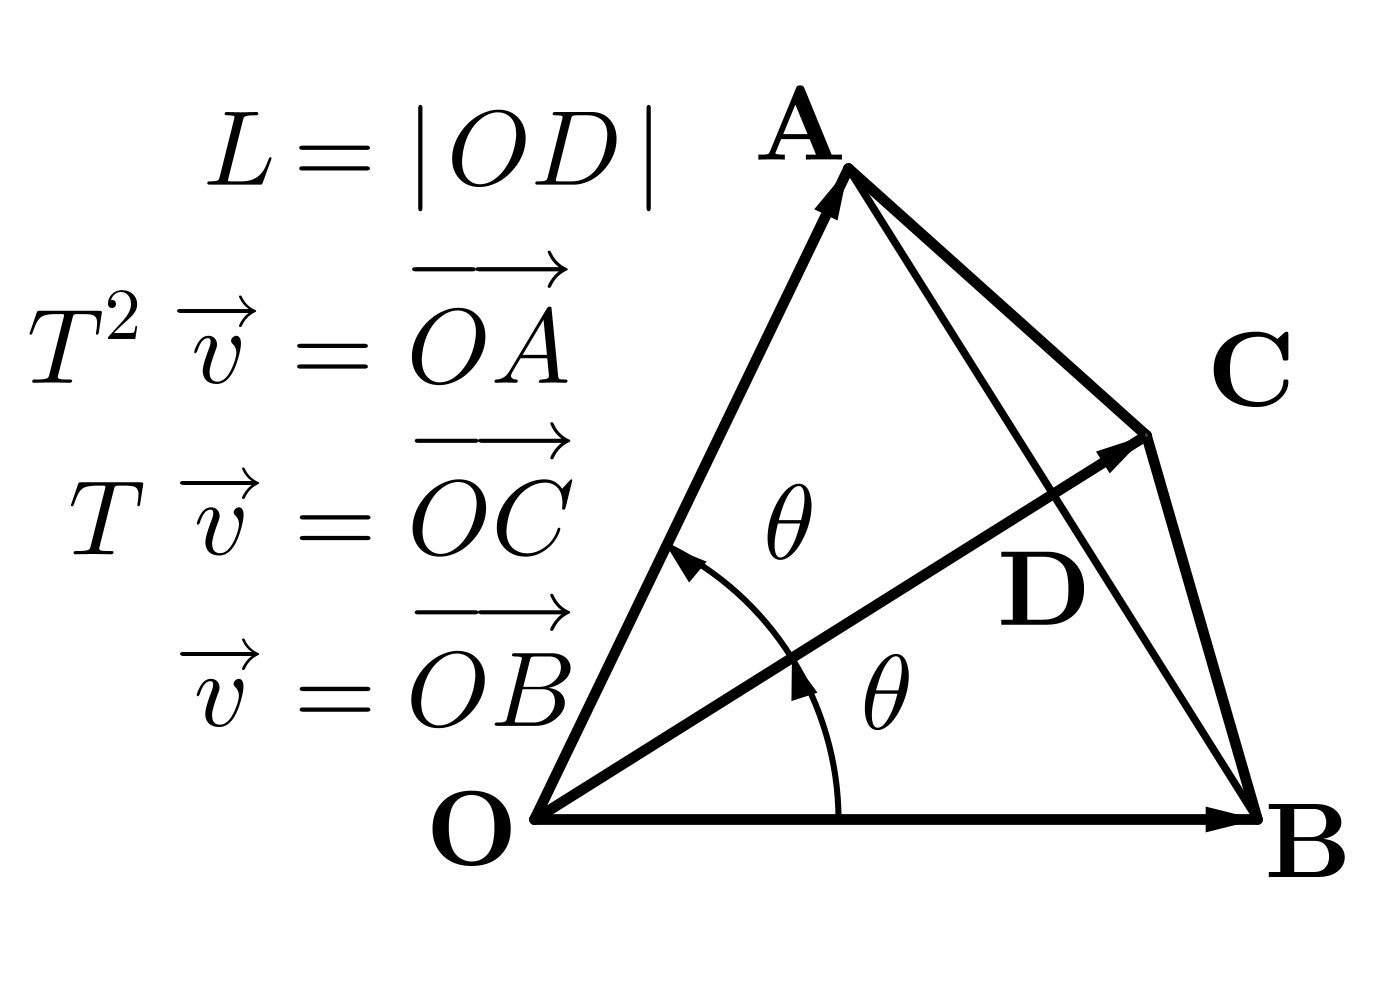
\includegraphics[width=4.4cm,height=3.2cm,scale=0.22]{diagram5BI-1.png}\par\vspace{-70pt}\quad
\hspace{180pt}{$\MathLeftMid{l}{Tv=\Frac{\left|\overset{\rightarrow}{v}\right|}{2L}\Par{T^2 v+v}\Rightarrow T=\Frac{\left|\overset{\rightarrow}{v}\right|}{2L}\Par{T^2+I}\\\vspace{8pt} L=\left|\overset{\rightarrow}{v}\right|\cos\theta\Rightarrow\Frac{\left|\overset{\rightarrow}{v}\right|}{2L}=\Frac{1}{2\cos\theta}}$}\par\quad
Hence $p\Par{T}=T^2-2\cos\theta\, T+I=0$ and $z^2-2\cos\theta\;z+1$ is the min poly of $T.$\PfEnd\vspace{6pt}\quad
\Or Let $\Par{e_1,e_2}$ be the std bss of $\Rbb^2.$ We use the pattern shown in [8.44].\par\quad
Becs $Te_1=\cos\theta\;e_1+\sin\theta\;e_2,\;T^2e_1=\cos2\theta\;e_1+\sin2\theta\;e_2.$\par\vspace{2pt}\quad
Thus \;$ce_1+bTe_1=-T^2 e_1\Longleftrightarrow{}${\small$\begin{pmatrix}
	1 & \cos\theta\\
	0 & \sin\theta
\end{pmatrix}\begin{pmatrix}
	c \\ b
\end{pmatrix}$}${}={}${\small$\begin{pmatrix}
-\cos2\theta\\
-\sin2\theta
\end{pmatrix}$}. Now $\det=\sin\theta\neq 0,c=1,b=2\cos\theta.$\PfEnd\vspace{12pt}\quad
\Or $\Mt[\BigPar]{T,\Par{e_1,e_2}}={}${\small$\begin{pmatrix}\Blind{-}\cos\theta & \sin\theta\\-\sin\theta & \cos\theta
\end{pmatrix}$}. By (4E 11), the min poly is $\Par{z\pm 1}$ or $\Par{z^2-2\cos\theta\,z+1}.$\PfEnd
\SepLine

\ProblemBnoor{\hypertarget{5BI4e11}{4E 11}}{
	\TextB{Supp $V$ is 2\hspace{1pt}-\hspace{1pt}dim, $T\in\Lm{V}$, and $\Mt{T,B_V}={}${\large$\begin{pmatrix} a & c\\ b & d\end{pmatrix}.$}\vspace{-8pt}}
	(a) \TextB{Show $T^2 - \Par{a + d}T + \Par{ad - bc}I = 0.$}
	(b) \TextB{Show the min poly of $T$ equals}
	\TextB{\FontNorm\centerline{$\MathLeftBrace{l}{z-a\qquad\qquad\qquad\qquad\qquad$ if $b=c=0$ and $a=d$,$\\ z^2-\Par{a+d}z+\Par{ad-bc}\quad$ \,\,othws.$}$}}
}\par\quad
(a) Supp the bss is $\Par{v,w}$. Becs $\MathLeftBrace{l}{Tv=av+bw\Rightarrow\Par{T-aI}v=bw,$ then apply $\Par{T-dI}$ to both sides. $\\ Tw=cv+dw\Rightarrow \Par{T-dI}w=cv,$ then apply $\Par{T-aI}$ to both sides. $}$\par\vspace{6pt}\quad\Ha
Hence $\Par{T-aI}\Par{T-dI}=bc I\Rightarrow T^2 - \Par{a + d}T + \Par{ad - bc}I = 0.$\par\quad
(b) If $b=c=0$ and $a=d.$ Then $\Mt{T}=${\small$\begin{pmatrix}a & 0\\ 0 & a\end{pmatrix}$}$=a\Mt{I}$. Thus $T=aI.$ Hence the min poly is $z-a.$\par\quad\Hb
Othws, by (a), $z^2-\Par{a+d}z+\Par{ad-bc}$ is a poly multi of the min poly.\par\quad\Hb
Now we prove that $T\not\in\Span{I},$ so that then the min poly of $T$ has exactly deg $2.$\par\quad\Hb
( At least one of the asum of (I),(II) below is true. )\par\quad\Hb
(I) Supp $a=d,$ then $Tv=av+bw\not\in\Span{v},Tw=cv+aw\not\in\Span{w}.$\par\qquad
(II) Supp at most one of $b,c$ is not $0.$ If $b=0,$ then $Tw\not\in\Span{w};$ If $c=0,$ then $Tv\not\in\Span{v}.$\PfEnd
\SepLine

\ProblemB{
	\TextB{Supp $S,T\in\Lm{V},S$ is inv, and $p\in\PoFi$. Prove $Sp\Par{TS}=p\Par{ST}S.$}
}\par\quad
We prove $S\Par{TS}{^m}=\Par{ST}{^m} S$ for each $m\in\Nbb\,$ by induc.\par\quad
(i) If $m=0,1.$ Then $S\Par{TS}{^0}=I=\Par{ST}{^0}S;\;S\Par{TS}{^1}=\Par{ST}S.$\par\quad\Endi
(ii) If $m>1.$ Asum $S\Par{TS}{^m}=\Par{ST}{^m} S.$\par\quad\Hii
Then $S\Par{TS}{^{m+1}}=S\Par{TS}{^m}\Par{TS}=\Par{ST}{^m} STS=\Par{ST}{^{m+1}}S.$\par\quad
Hence $\forall p\in\PoFi,Sp\Par{TS}=\sum_{k=1}^ma_kS\Par{TS}{^k}=\sum_{k=1}^ma_kp\Par{ST}{^k}S=\Sbra{\sum_{k=1}^ma_k\Par{TS}{^k}}S.$\PfEnd\vspace{2pt}
\AComm $p\Par{TS} = S^{-1} p\Par{ST}S,\;p\Par{ST} = Sp\Par{TS}S^{-1}.$\par
\ACoro \ProblemN[]{\hypertarget{5BI5}{5}}{
	Becs $S$ is inv, $T\in\Lm{V}$ is arb $\Longleftrightarrow R=ST$ is arb.\TextN{}
	{\IndentCorollary} Hence $\forall R\in\Lm{V},$ inv $S\in\Lm{V},p\Par{S^{-1}RS}=S^{-1}p\Par{R}S.$\TextN{\vspace{-4pt}}
}\SepLine

\ProblemBnoor{\hypertarget{5BI4e7}{4E 5.B.7}}{
	\TextB{Supp $S, T\in\Lm{V}.$ Let $p,q$ be the min polys of $ST,TS$ respectly.}
	(a) \TextB{If $V=\Fbb^2.$ Give an exa suth $p\neq q;$ \;{\large\tgnr(b)} If $S$ or $T$ is inv. Prove $p=q.$}
}\par\quad
(a) %Let $V=\Fbb^{\infty},$ $S\in\Lm{\Fbb^\infty}$ is the forwd shift optor, $T\in\Lm{\Fbb^\infty}$ is the backwd shift optor.\par\quad\Ha
%Then $ST(x_1,x_2,x_3,\dots)=(0,x_2,x_3,\dots)\Rightarrow 0,1$ are all the eigvals of $ST,$ $(ST)^2-(ST)=0.$\par\quad\Ha
%$TS(x_1,x_2,\dots)=(x_1,x_2,\dots)\Rightarrow 1$ is the only eigval of $TS,$ $TS=I.$\par\quad\Ha
Define $S$ by $S\Par{x,y}=\Par{x,x}.$ Define $T$ by $T\Par{x,y}=\Par{0,y}.$\par\quad\Ha
Then $ST\Par{x,y}=0,\,\,TS\Par{x,y}=\Par{0,x}$ for all $\Par{x,y}\in\Fbb^2.$ Thus $ST=0\neq TS$ and $\Par{TS}^2=0.$\par\quad\Ha
Hence the min poly of $ST$ does not equal to the min poly of $TS.$\par\quad
(b) Supp $S$ is inv. Becs $p,q$ are monic.\par\quad\Hb
$\MathRightBrace{l}{$
$p\Par{ST}=0=S p\Par{TS}S^{-1}\Rightarrow p\Par{TS}=0,p$ is a poly multi of $q\\ $
$q\Par{TS}=0=S^{-1} q\Par{ST}S\Rightarrow q\Par{ST}=0,q$ is a poly multi of $p$
$}\Rightarrow p=q.$\par\vspace{6pt}\quad\Hb
Reversing the roles of $S$ and $T$, we conclude that if $T$ is inv, then $p=q$ as well.\PfEnd
\SepLine

\ProblemN{\hypertarget{5BI11}{11}}{
	\TextNL{Supp $\Fbb = \Cbb,$ $T\in\Lm{V}, p\in\PoCi$, and $\alpha\in\Cbb.$}
	\TextNL{Prove $\alpha$ is an eigval of $p\Par{T}$ $\Longleftrightarrow$ $\alpha = p\Par{\lambda}$ for some eigval $\lambda$ of $T$.}
}\par\quad
(a) Supp $\alpha$ is an eigval of $p\Par{T}\Leftrightarrow \BigPar{p\Par{T}-\alpha I}$ is not inje.\par\quad\Ha
Write $p\Par{z}-\alpha=c\Par{z-\lambda_1}\cdots\Par{z-\lambda_m}\Rightarrow p\Par{T}-\alpha I=c\Par{T-\lambda_1 I}\cdots\Par{T-\lambda_m I}.$\par\quad\Ha
By {\TIPS}, $\exists\,\Par{T-\lambda_j I}$ not inje. Thus $p\Par{\lambda_j}-\alpha=0.$\par\quad
(b) Supp $\alpha=p\Par{\lambda}$ and $\lambda$ is an eigval of $T$ with an eigvec $v.$ Then $p\Par{T}v=p\Par{\lambda}v=\alpha v.$\PfEnd\vspace{3pt}\quad\Hb
\Or Define $q$ by $q\Par{z}=p\Par{z}-\alpha.$ $\lambda$ is a zero of $q.$\par\quad\Hb
Becs $q\Par{T}v=\BigPar{p\Par{T}-\alpha I}v=q\Par{\lambda}v=\BigPar{p\Par{\lambda}-\alpha}v=0.$\par\quad\Hb
Hence $q\Par{T}$ is not inje $\Rightarrow \BigPar{p\Par{T}-\alpha I}$ is not inje.\PfEnd
\SepLine

\ProblemNnoor{\hypertarget{5BI12}{12}}{4E 6}{
	\TextNL{Give a $T\in\Lm{\Rbb^2}$ that shows the result above does not hold if $\Cbb$ is replaced with $\Rbb$.}
}\par\quad
Define $T\in\Lm{\Rbb^2}$ by $T\Par{w,z}=\Par{-z,w}.$\par\quad
By Exe (4E 5.B.11), $\Mt[\BigPar]{T,\Par{\Par{1,0},\Par{0,1}}}=\,${\small$\begin{pmatrix}0 & -1\\ 1 & 0\end{pmatrix}$}$\Rightarrow$ the min poly of $T$ is $z^2+1.$\par\quad
Define $p$ by $p\Par{z}=z^2.$ Then $p\Par{T}=T^2=-I.$ Thus $p\Par{T}$ has eigval $-1.$\par\quad
While $\nexists\,\lambda\in\Rbb$ suth $-1=p\Par{\lambda}=\lambda^2.$\PfEnd
\SepLine

\ProblemBnoor{\hypertarget{5BI4e17}{4E 17}}{
	\TextB{Supp $V$ is finide, $p$ is min of $T\in \Lm{V},$ and $\lambda\in\Fbb.$}
	\TextB{Show $q\Par{z}=p\Par{z+\lambda}$ is min of $\Par{T-\lambda I}.$}
}\par\quad
$q\Par{T-\lambda I}=0\Rightarrow q$ is poly multi of the min poly of $\Par{T-\lambda I}.$\par\quad
Supp the deg of the min poly of $\Par{T-\lambda I}$ is $n,$ and the deg of the min poly of $T$ is $m.$\par\quad
%Write $q(z)=p(z+\lambda)=a_0+a_1(z+\lambda)+\dots+a_{m-1}(z+\lambda)^{m-1}+(z+\lambda)^m.$\par\quad
By definition of min poly,\par\quad
$n$ is the smallest suth $\Par{T-\lambda I}^n\in\Span{I,\Par{T-\lambda I},\dots,\Par{T-\lambda I}^{n-1}};$\par\quad
$m$ is the smallest suth $T^m\in\Span{I,T,\dots,T^{m-1}}.$\par\quad
又 $T^k\in\Span{I,T,\dots,T^{k-1}}\Longleftrightarrow \Par{T-\lambda}^k\in\Span{I,\Par{T-\lambda I},\dots,\Par{T-\lambda I}^{k-1}}.$\par\quad
Thus $n=m.$ 又 $q$ is monic. By the uniqnes of min poly.\PfEnd
\SepLine

\ProblemBnoor{\hypertarget{5BI4e18}{4E 18}}{
	\TextB{Supp $V$ is finide, $p$ is min of $T\in \Lm{V},\lambda\neq 0.$ Show $q\Par{z} = \lambda^{\deg p} p\BigPar{{z}\big/{\lambda}}$ is min of $\lambda T.$}
}\par\quad
$q\Par{\lambda T}=\lambda^{\deg p}p\Par{T}=0\Rightarrow q$ is a poly multi of the min poly of $\lambda T.$\par\quad
Supp the deg of the min poly of $\lambda T$ is $n,$ and the deg of the min poly of $T$ is $m.$\par\quad
By definition of min poly,\par\quad
$n$ is the smallest suth $\Par{\lambda T}^n\in\Span{\lambda I,\lambda T,\dots,\Par{\lambda T}^{n-1}};$\par\quad
$m$ is the smallest suth $T^m\in\Span{I,T,\dots,T^{m-1}}.$\par\quad
又 $\Par{\lambda T}^k\in\Span{\lambda I,\lambda T,\dots,\Par{\lambda T}^{k-1}}\Longleftrightarrow T^k\in\Span{I,T\dots,T^{k-1}}.$\par\quad
Thus $n=m.$ 又 $q$ is monic. By the uniqnes of min poly.\PfEnd
\SepLine

\ProblemNnoor{\hypertarget{5BI18}{18}}{\hypertarget{5BI4e15}{4E 15}}{
	\TextNL{Supp $V$ is a finide complex vecsp with $\dim V > 0$ and $T\in\Lm{V}$.}
	\TextNL{Define $f:\Cbb\rightarrow\Rbb$ by $f\Par{\lambda} = \dim \Range\Par{T-\lambda I}$. Prove $f$ is not continuous.}
}Note that $V$ is finide.\par\quad
Let $\lambda_0$ be an eigval of $T.$ Then $\Par{T-\lambda_0 I}$ is not surj. Hence $\dim\Range\Par{T-\lambda_0 I}<\dim V.$\par\quad
Becs $T$ has finily many eigvals. There exis a seq of number $\Bra{\lambda_n}$ suth $\lim\limits_{n\rightarrow\infty}\lambda_n=\lambda_0$.\par\quad
And $\lambda_n$ is not an eigval of $T$ for each $n\Rightarrow\dim\Range\Par{T-\lambda_n I}=\dim V\neq \dim\Range\Par{T-\lambda_0 I}.$\par\quad
Thus $f\Par{\lambda_0}\neq \lim\limits_{n\rightarrow\infty}f\Par{\lambda_n}.$\PfEnd
\SepLine

\ProblemBnoor{\hypertarget{5BI4e9}{4E 5.B.9}}{
	\TextB{Supp $T\in\Lm{V}$ is suth wrto some bss of $V$,}
	\TextB{all ent of the matrix of $T$ are rational numbers.}
	\TextB{Explain why all coeffs of the min poly of $T$ are rational numbers.}
}\par\quad
Let $\Par{v_1,\dots,v_n}$ denote the bss suth $\Mt[\BigPar]{T,\Par{v_1,\dots,v_n}}_{j,k}=A_{j,k}\in\Qbb$ for all $j,k=1,\dots,n$.\par\quad
Denote $\Mt[\BigPar]{v_j,\Par{v_1,\dots,v_n}}$ by $x_j$ for each $v_j.$\par\quad
Supp $p$ is the min poly of $T$ and $p\Par{z}=z^m+\dots+c_1 z+c_0.$ Now we show each $c_j\in\Qbb.$\par\quad
Note that $\forall s\in\Nbp,\Mt{T^s}=\Mt{T}^s=A^s\in\Qbb^{n,n}$ and $T^s v_k=A^s_{1,k} v_1+\dots+A^s_{n,k}v_n$ for all $k\in\Bra{1,\dots,n}.$\par\vspace{6pt}\quad
Thus $\MathLeftBrace{l}{
\Mt{p\Par{T}v_1}=\Par{A^m+\dots+c_1 A+c_0 I}x_1=\sum\limits_{j=1}^n\Par{A^m+\dots+c_1 A+c_0 I}_{j,1}x_j=0;\\ \qquad\qquad\vdots \\
\Mt{p\Par{T}v_n}=\Par{A^m+\dots+c_1 A+c_0 I}x_n=\sum\limits_{j=1}^n\Par{A^m+\dots+c_1 A+c_0 I}_{j,n}x_j=0;
}$\par\quad
More clearly, $\MathLeftBrace{l}{
\Par{A^m+\dots+c_1 A+c_0 I}_{1,1}=\cdots=\Par{A^m+\dots+c_1 A+c_0 I}_{n,1}=0;\\\hspace{130pt}\vdots\hspace{8pt}\ddots\hspace{8pt}\vdots\\
\Par{A^m+\dots+c_1 A+c_0 I}_{1,n}=\cdots=\Par{A^m+\dots+c_1 A+c_0 I}_{n,n}=0;
}$\par\quad
Hence we get a system of $n^2$ liney equations in $m$ unknowns $c_0,c_1,\dots,c_{m-1}.$\par\quad
We conclude that $c_0,c_1,\dots,c_{m-1}\in\Qbb.$\PfEnd
\SepLine

\ProblemBnoor{\OR (\hypertarget{5BI4e16}{4E 5.B.16}), \OR (8.C.18)}[\Sbra]{
	\TextB{Supp $a_0 ,\dots, a_{n-1}\in\Fbb.$ Let $T$ be the optor on $\Fbb^n$ suth\vspace{2pt}}
	\TextB{$\Mt{T}=\,${\normalsize$\begin{pmatrix}
	0 &   &        &  &   & -a_0     \\
	1 & 0 &        &  &   & -a_1     \\
	  & 1 & \ddots &  &   & \vdots   \\
	  &   & \ddots &  & 0 & -a_{n-2} \\
	0 &   &        &  & 1 & -a_{n-1}
\end{pmatrix} $}, wrto the std bss $\Par{e_1,\dots,e_n}$.\vspace{4pt}}
	\TextB{Show the min poly of $T$ is $\,p\,$ defined by $p\Par{z}=a_0 + a_1 z + \dots + a_{n-1} z^{n-1} + z^n$.}
	\vspace{-2pt}\TextB{\small $\Mt{T}$ is called the {\tgsc companion matrix} of the poly above. This exercise shows that every monic poly is the min poly of some optor.}
	\vspace{-2pt}\TextB{\small Hence a formula or an algo that could produce exact eigvals for each optor on each $\Fbb^n$ could then produce exact zeros for}
	\vspace{-2pt}\TextB{\small each poly  $[$ by 8.36(b) $]$. Thus there is no such formula or algo. However, efficient numeric methods exis for obtaining very good}
	\TextB{\small approximations for the eigvals of an optor.}
}Note that $\Par{e_1,Te_1,\dots,T^{n-1}e_1}$ is liney indep. 又 The deg of min poly is at most $n.$\par\quad
$T^n e_1=\cdots=T^{n-k}e_{1+k}=\cdots=T e_n=-a_0 e_1-a_1 e_2-a_2 e_3-\dots-a_{n-1}e_n$\par
$=\Par{-a_0 I-a_1 T-a_2 T^2-\dots-a_{n-1}T^{n-1}}e_1.$ Thus $p\Par{T}e_1=0=p\Par{T}e_j$ for each $e_j=T^{j-1}e_1.$\PfEnd
\SepLine

\BulletPointX{\Large\textsc{Eigenvalues On Odd-Dimensional Real Vector Spaces}}\par
\ProblemB{
	\textsc{Even-Dimensional Null Space}\TextB{}
	\TextB{Supp $\Fbb=\Rbb,$ $V$ is finide, $T\in\Lm{V}$ and $b, c\in\Rbb$ with $b^2 < 4c$.}
	\TextB{Prove $\dim\Null\Par{T^2 + bT + cI}$ is an even number.}
}\par\quad
Denote $\Null\Par{T^2 + bT + cI}$ by $R.$ Then $T\mmid_R+bT\mmid_R+cI_R=\Par{T+bT+cI}\mmid_R=0\in\Lm{R}.$\par\quad
Supp $\lambda$ is an eigval of $T_R$ with an eigvec $v\in R.$\par\quad
Then $0=\Par{T\mmid_R^2+bT\mmid_R+cI_R}\Par{v}=\Par{\lambda^2+\lambda b+c}v=\BigPar{\Par{\lambda+b}^2+c-\Frac{b^2}{4}}v.$\par\quad
Becs $c-\Frac{b^2}{4}>0$ and we have $v=0.$ Thus $T_R$ has no eigvals.\par\quad
Let $U$ be invarsp of $R$ that has the largest, even dim among all invarsps.\par\quad
Asum $U\neq R.$ Then $\exists\,w\in R$ but $w\not\in U.$ Let $W$ be suth $\Par{w,T\mmid_R w}$ is a bss of $W.$\par\quad
Becs $T\mmid_R^2 w=-bT\mmid_R w-cw\in W.$ Hence $W$ is invarsp of dim $2.$\par\quad
Thus $\dim \Par{U+W}=\dim U+2-\Dim\Par{U\cap W},$ where $U\cap W=\zeroSubs,$\par\qquad\qquad
for if not, becs $w\not\in U,T\mmid_R w\in U,$\par\qquad\qquad $U\cap W$ is invard $T\mmid_R$ of one dim ( impossible becs $T\mmid_R$ has no eigvecs ).\par\quad
Hence $U+W$ is even-dim invarsp under $T\mmid_R$, ctradic the max of $\dim U.$\par\quad
Thus the asum was incorrect. Hence $R=\Null\Par{T^2+bT+cI}=U$ has even dim.\PfEnd
\SepLine

\ProblemB{
	\textsc{Operators On Odd-Dimensional Vector Spaces Have Eigenvalues}\TextB{}
	(a) \TextB{Supp $\Fbb=\Cbb.$ \tgnr\large Then by [5.21], done.}
	(b) \TextB{Supp $\Fbb=\Rbb,$ $V$ is finide, and $\dim V=n$ is an odd number.}
	\Hb\TextB{Let $T\in\Lm{V}$ and the min poly is $\,p\,$. Prove $T$ has an eigval.}
}\par\quad
(i) If $n=1,$ then done.\par\quad\Endi
(ii) Supp $n\geqslant 3.$ Asum every optor, on odd-dim vecsps of dim less than $n,$ has an eigval.\par\quad\Hii
If $p$ is a poly multi of $\Par{x - \lambda}$ for some $\lambda\in\Rbb,$ then by [8.49] $\lambda$ is an eigval of $T$ and done.\par\quad\Hii
Now supp $b, c\in\Rbb$ suth $b^2 < 4c$ and $p$ is a poly multi of $x^2 + bx + c$ (see [4.17]).\par\quad\Hii
Then $\exists\,q\in\PoRi$ suth $p\Par{x} = q\Par{x}\Par{x^2 + bx + c}$ for all $x\in\Rbb.$\par\quad\Hii
Now $0 = p\Par{T} = \BigPar{q\Par{T}}\Par{T^2 + bT + cI},$ which means that $q\Par{T}\mmid_{\Range\Par{T^2+bT+cI}}=0.$\par\quad\Hii
Becs $\deg q < \deg p$ and $p$ is the min poly of $T$, hence $\Range\Par{T^2 + bT + cI}\neq V$.\par\quad\Hii
又 $\dim V$ is odd and $\dim\Null\Par{T^2 +bT+cI}$ is even ( by our previous result ).\par\quad\Hii
Thus $\dim V - \dim \Null\Par{T^2 + bT + cI}=\dim \Range\Par{T^2 + bT + cI}$ is odd.\par\quad\Hii
By [5.18], $\Range\Par{T^2 + bT + cI}$ is invarsp of $V$ under $T$ that has odd dim less than $n.$\par\quad\Hii
Our induc hypo now implies that $T\mmid_{\Range\Par{T^2 + bT + cI}}$ has an eigval.\par\quad
By induc.\PfEnd
\SepLine

\ProblemBnoor{\hypertarget{5BI2e24}{2E 24}}{
	\TextB{Supp $\Fbb=\Rbb,T\in\Lm{V}$ has no eigvals. Prove every invarspd $T$ is even-dim.}
}\par\quad
Supp $U$ is such a subsp. Then $T\mmid_U\in\Lm{U}.$
We prove by ctradic.\par\quad
If $\dim U$ is odd, then $T\mmid_U$ has an eigval and so is $T,$ so that $\exists$ invarsp of $1$ dim, ctradic.\PfEnd
\SepLine

\ProblemBnoor{\hypertarget{5BI4e29}{4E 29}}{
	\TextB{Show every optor on a finide vecsp of dim $\geq 2$ has a $2$-dim invarsp.}
}\par\quad
Using induc on $\dim V.$\par\quad
(i) $\dim V=2,$ done.\par\quad\Endi
(ii) $\dim V>2.$ Asum the desired result is true for vecsp of smaller dim.\par\quad\Hii
Supp $p$ is the min poly of deg $m$ and $p\Par{z}=\Par{z-\lambda_1}\cdots\Par{z-\lambda_m}.$\par\quad\Hii
If $\,T=\lambda I\,\Par{\,\Leftrightarrow m=1\,\vee\,m=-\infty\,},$ then done. ( $m\neq 0$ becs $\dim V\neq 0.$ )\par\quad\Hii
Now define a $q$ by $q\Par{z}=\Par{z-\lambda_1}\Par{z-\lambda_2}$.\par\quad\Hii
By asum, $T\mmid_{\nullp q\Par{T}}$ has invarsp of dim $2.$\PfEnd
\SepLine

\ChEnd

% 6h
\ChDecl{Ch5BII}{5.B: II}{}\orMode{\hLk{5BII9}{9}\;\;\hLk{5BII14}{14}\;\;\hLk{5BII15}{15}\;\;\hLk{5BII20}{20}\;\;|\;\;\hLk{5BII4e1}{4E: 1,}\;\;\hLk{5BII4e2}{2,}\;\;\hLk{5BII4e3}{3,}\;\;\hLk{5BII4e4}{4,}\;\;\hLk{5BII4e5}{5,}\;\;\hLk{5BII4e6}{6,}\;\;\hLk{5BII4e7}{7,}\;\;\hLk{5BII4e8}{8,}\;\;\hLk{5BII4e9}{9,}\;\;\hLk{5BII4e10}{10}\;\;\hLk{5BII4e11}{11,}\;\;\hLk{5BII4e12}{12,}\;\;\hLk{5BII4e13}{13,}\;\;\hLk{5BII4e14}{14}}{[1]: ; [2]: ; [3]: .}

\ProblemBnoor{\hypertarget{5BII4e1}{4E 5.C.1}}{
	\TextB{Supp $T^2$ has up-trig matrix. Give a countexa\hspace{1pt}$:$ $T$ has up-trig matrix.}
}
\SepLine

\ProblemBnoor{\hypertarget{5BII4e2}{4E 5.C.2}}{
	\TextB{Supp $A$ and $B$ are up-trig matrices of the same size,}
	\TextB{with $\alpha_1 , \dots , \alpha_n$ on the diag of $A$ and $\beta_1 , \dots , \beta_n$ on the diag of $B$.}
	(a) \TextB{Show $A + B$ up-trig with $\alpha_1 + \beta_1 , \dots , \alpha_n + \beta_n$ on the diag.}
	(b) \TextB{Show $AB$ up-trig with $\alpha_1 \beta_1 , \dots , \alpha_n \beta_n$ on the diag.}
}
\SepLine

\ProblemBnoor{\hypertarget{5BII4e3}{4E 5.C.3}}{
	\TextB{Supp $T$ inv, $B_V=\Par{v_1,\dots,v_n},$ $\Mt{T}=A$ is up-trig,}
	\TextB{with $\lambda_1,\dots,\lambda_n$ on diag. Show $A^{-1}$ is also up-trig, with $\lambda_1^{-1},\dots,\lambda_n^{-1}$ on diag.}
}
\SepLine

\ProblemNnoor{\hypertarget{5BII9}{9}}{\hypertarget{5BII4e7}{4E 5.C.7}}{
	\TextN{Supp $V$ is finide, and $v \in V$.}
	(a) \TextN{Prove $\exists\,!$ monic $p_v$ of smallest deg suth $p_v\Par{T}v = 0$.}
	(b) \TextN{Prove the min poly of $T$ is a poly multi of $p_v$.}
}
\SepLine

\ProblemNor{\hypertarget{5BII14}{14}}{\hypertarget{5BII4e4}{4E 5.C.4}}{
	\TextNL{Give an inv $T$ and a $B_V$ suth each $\Mt{T}{_{k,k}}=0.$}
}
\SepLine

\ProblemNor{\hypertarget{5BII15}{15}}{\hypertarget{5BII4e5}{4E 5.C.5}}{
	\TextNL{Give a non-inv $T$ and a $B_V$ suth each $\Mt{T}{_{k,k}}\neq 0.$}
}
\SepLine

\ProblemNor{\hypertarget{5BII20}{20}}{\hypertarget{5BII4e6}{4E 5.C.6}}{
	\TextNL{Supp $\Fbb=\Cbb,$ $V$ is finide, and $k\in\Bra{1,\dots,\dim V}.$}
	\TextNL{Prove $V$ has a $k$\hspace{1pt}-\hspace{1pt}dim subsp invard $T$.}
}\par
\SepLine

\ProblemBnoor{\hypertarget{5BII4e8}{4E 5.C.8}}{
	\TextB{Supp $V$ is finide, and $\exists\,v\in V\nonzero$ suth $T^2 v + 2Tv = -2v$.}
	(a) \TextB{Supp $\Fbb=\Rbb.$ Prove $\nexists\,B_V$ suth $\Mt{T}$ up-trig.}
	(b) \TextB{Supp $\Fbb=\Cbb,$ and $\exists\,B_V$ suth $A=\Mt{T}$ up-trig. Prove $-1+\i$ or $-1-\i$ on the diag of $A$.}
}\par
\SepLine

\ProblemBnoor{\hypertarget{5BII4e9}{4E 5.C.9}}{
	\TextB{Supp $B\in\Fbb^{n,n}$ with complex ent.}
	\TextB{Prove $\exists$ inv $A\in\Fbb^{n,n}$ with complex ent suth $A^{-1} BA$ is up-trig.}
}\par

\par
\SepLine

\ProblemBnoor{\hypertarget{5BII4e10}{4E 5.C.10}}{
	\TextB{Supp $B_V=\Par{v_1,\dots,v_n}.$ Show the following are equi\hspace{1pt}$:$}
	(a) \TextB{$\Mt{T,B_V}$ lower trig. \, {\tgnr\large(b)} Each $\Span{v_k,\dots,v_n}$ invard $T.$ \, {\tgnr\large(c)} Each $Tv_k\in\Span{v_k,\dots,v_n}.$}
}\par
\SepLine

\ProblemBnoor{\hypertarget{5BII4e11}{4E 5.C.11}}{
	\TextB{Supp $\Fbb=\Cbb,$ $V$ is finide. Prove $\exists\,B_V$ suth $\Mt{T}$ low-trig.}
}\par
\SepLine

\ProblemBnoor{\hypertarget{5BII4e12}{4E 5.C.12}}{
	\TextB{Supp $V$ is finide, $U$ invarspd $T,$ and $\Mt{T}$ is up-trig for some $B_V.$}
	(a) \TextB{Prove $\Mt{T\mmid_U}$ up-trig for some $B_U$. \, {\tgnr\large(b)} Prove $\Mt{T\XSlash U}$ up-trig for some $B_{V\XSlash U}.$}
}
\SepLine

\ProblemBnoor{\hypertarget{5BII4e13}{4E 5.C.13}}{
	\TextB{Supp $V$ is finide, $U$ invarspd $T$ suth $T\mmid_U,T\XSlash U$ up-trig. Prove $T$ up-trig.}
}
\SepLine

\ProblemBnoor{\hypertarget{5BII4e14}{4E 5.C.14}}{
	\TextB{Supp $V$ is finide. Prove $T$ up-trig $\Longleftrightarrow$ $T\apostrophe$ up-trig.}
}
\SepLine

\ChEnd

\ChDecl{Ch5C}{5.C} % 10h

XXXX


\par
\SepLine

\ChEnd
\ChDecl{Ch5E}{5.E* [4E]}{}\orMode{\hLk{5E1}{1}\;\;\hLk{5E2}{2}\;\;\hLk{5E3}{3}\;\;\hLk{5E4}{4}\;\;\hLk{5E5}{5}\;\;\hLk{5E6}{6}\;\;\hLk{5E7}{7}\;\;\hLk{5E8}{8}\;\;\hLk{5E9}{9}\;\;\hLk{5E10}{10}}{}
% 0.5h/4h

\ProblemN{1}{
	\TextN{Give commu optors $S,T\in\Fbb^4$ suth $\exists$ invarspd $S$ but not $T$ and $\exists$ invarspd $T$ but not $S$.}
}
\par
\SepLine

\ProblemN{2}{
	\TextN{Supp $\mathcal{E}$ is a subset of $\Lm{V}$ and every elem of $\mathcal{E}$ is diag.}
	\TextN{Prove $\exists\,B_V$ suth each elem of $\mathcal{E}$ diag $\Longleftrightarrow$ each pair of elems of $\mathcal{E}$ commu.}
}\par
\SepLine

\ProblemN{3}{
	\TextN{Supp $S, T\in\Lm{V}$ are suth $ST = TS$. Supp $p\in\PoFi$.}
	(a) \TextN{Prove $\nullp p\Par{S}$ is invard $T$. \, {\tgnr\large(b)} Prove $\rangep p\Par{S}$ is invard $T$.}
}\par
\SepLine

\ProblemN{4}{
	\TextN{Prove or give a countexa\hspace{1pt}$:$ A diag matrix $A$ and up-trig matrix $B$ of the same size commu.}
}\par
\SepLine

\ProblemN{5}{
	\TextN{Prove a pair of optors on a finide vecsp commu $\Longleftrightarrow$ their dual optors commu.}
}\par
\SepLine

\ProblemN{6}{
	\TextN{Supp $V$ is a finide complex vecsp and $S, T\in\Lm{V}$ commu.}
	\TextN{Prove $\exists\,\alpha,\lambda\in\Cbb$ suth $\Range\Par{S -\alpha I} + \Range\Par{T -\lambda I}\neq V$.}
}\par
\SepLine

\ProblemN{7}{
	\TextN{Supp $V$ is a complex vecsp, $S\in\Lm{V}$ is diag, and $T$ commu with $S$.}
	\TextN{Prove $\exists\,B_V$ suth $S$ diag $T$ up-trig.}
}\par
\SepLine

\ProblemN{8}{
	\TextN{Supp $m = 3$ in [5.72] and $D_x , D_y$ are the commu partial diff optors on $\Po_3\Par{\Rbb^2}$ from [5.72].}
	\TextN{Find a bss of $\Po_3\Par{\Rbb^2}$ suth $D_x$ and $D_y$ each up-trig.}
}\par
\SepLine

\ProblemN{9}{
	\TextN{Supp $V$ is a finide nonzero complex vecsp.}
	\TextN{Supp that $\mathcal{E}\subseteq\Lm{V}$ is suth $S$ and $T$ commu for all $S, T\in\mathcal{E}$.}
	(a) \TextN{Prove $\exists$ eigvec $v\in V$ for every elem of $\mathcal{E}$.}
	(b) \TextN{Prove $\exists$ a bss of $V$ wrto which every elem of $\mathcal{E}$ has up-trig matrix.}
}\par
\SepLine

\ProblemN{10}{
	\TextNL{Give commu optors $S, T$ on a finide real vecsp suth}
	\TextNL{$S + T$ has a eigval that does not equal an eigval of $S$ plus an eigval of $T$}
	\TextNL{and $ST$ has a eigval that does not equal an eigval of $S$ times an eigval of $T$.}
}
\par
\SepLine
\ChEnd

